\section{Disturbi dell'umore}

\subsection{Definizione disturbo dell'umore}

Le persone normali sperimentano quotidianamente delle \emph{fluttuazioni
del tono dell'umore}, del tutto fisiologiche, che sono in genere
collegate a degli eventi esterni al soggetto, e che rappresentano quindi
dei meccanismi dotati di una funzione adattativa, in quanto modulano la
spinta all'iniziativa, caratterizzano le risposte individuali e
favoriscono l'adozione di modelli comportamentali in rapporto ai
cambiamenti delle condizioni ambientali. Banalmente l'umore varia dal
lunedì mattina al venerdì pomeriggio e può variare anche nella stessa
giornata in maniera \emph{relativamente} imprevedibile.
``Relativamente'' perché le fluttuazioni sono connesse a stimoli
ambientali \emph{l'umore mantiene una certa reattività con l'ambiente}.
L'umore può variare a seconda che sia lunedì mattina o venerdì
pomeriggio ma non mi aspetto che questa variazione abbia un impatto così
devastante da non consentire di svolgere le abitudini quotidiane.

Quando però subentrano delle alterazioni dei meccanismi neurobiologici
che controllano l'umore, le oscillazioni possono diventare \emph{ampie},
\emph{prolungate}, o anche \emph{sproporzionate ed indipendenti rispetto
agli stimoli esterni}, perdendo in tal caso la loro funzione adattativa
e dando luogo a quelli che prendono appunto il nome di: \textbf{disturbi
dell'umore}.

Per disturbo intendiamo una condizione a cui corrispondono certe
manifestazioni cliniche con una certa durata ed a causa di queste
manifestazioni si comprometta la capacità di svolgere adeguatamente le
attività quotidiane da parte del soggetto colpito.

Le distimie sono disturbi ampiamente diffusi nella popolazione generale,
costituendo peraltro una delle cause di invalidità più comuni (dopo
l'infarto) anche perché questi disturbi possono purtroppo
\emph{associarsi} anche ad altre patologie psichiatriche e all'abuso di
alcol e di sostanze stupefacenti, e non bisogna dimenticare nemmeno
l'\emph{alto rischio di suicidio} che questi pazienti manifestano
durante il decorso della loro patologia (tra i suicidi, infatti, il
45-70\% è depresso, mentre fino al 15\% dei depressi tenta il suicidio).

\subsection{Classificazione disturbi dell'umore}

\begin{itemize}
\item
  Psicosi Manico-Depressiva
\item
  Depressione Somatogena-Psicogena
\item
  Depressione Psicotica-nevrotica
\item
  Depressione Endogena- Reattiva
\item
  Depressione Primaria-secondaria
\item
  Depressione Unipolare-bipolare
\end{itemize}

Il sistema di classificare i disturbi mentali è cominciato al termine
dell'Ottocento quando uno psichiatra tedesco Emil Kraepelin distinse tra
\textbf{demenza precoce e psicosi maniaco depressiva.} La distinzione
era legata al DECORSO DEL DISTURBO:

\begin{itemize}
\item
  che nel caso della \emph{\textbf{demenza precoce}} è cronico e
  progressivo e termina in una compromissione della personalità
  dell'individuo in età molto precoce, tale per cui era impossibile che
  questo potesse mantenere un livello di vita congruo alla propria età,
  al proprio ambiente di provenienza ed allo stato sociale;
\item
  nel caso della \emph{\textbf{psicosi maniaco depressiva}} si ha un
  andamento ciclico con episodi di malattia intervallati da periodi di
  benessere non associati ad un decadimento delle prestazioni del
  soggetto e della sua capacità di mantenere un certo livelo di vita in
  base ai presupposti prima elencati.

  La dicitura \textbf{`'maniaco-depressiva''} deriva dal riscontro di
  oscillazione dello stato clinico del paziente tra due polarità
  rappresentate da fasi depressive e fasi maniacali, con caratteristiche
  cliniche e sintomatologiche completamente opposte.

  Il termine \textbf{`'psicosi''} indicava la particolare gravità del
  disturbo.
\end{itemize}

Con l'avvento del pensiero freudiano si è cercato di distinguere la
depressione in base all'ORIGINE della stessa, se traesse origine da
alterazione endocrine o metaboliche oppure da un conflitto di tipo
psichico (\textbf{\emph{depressione somatogena} o \emph{psicogena}}.

Sempre sulla stessa scia della scuola freudiana deriva la distinzione
tra \textbf{\emph{depressione psicotica} e \emph{nevrotica},} dove per
psicotica si intendeva un disturbo grave al punto tale da compromettere
la percezione della realtà da parte dello stesso individuo e da fargli
vivere esperienze deliranti.

Successivamente la distinzione tra \textbf{\emph{depressione endogena} e
\emph{reattiva}} che imponeva una dicotomia tra EZIOLOGIE: l'una
prevedeva fattori eziologici endogeni, avulsi dalla realtà in cui si
relazionava il paziente, mentre l'altra indicava un'eziologia dipendente
da fattori scatenanti.

In seguito, si è cercato di distinguere le manifestazioni in due maxi-
categorie aspecifiche: \textbf{\emph{depressione} \emph{primaria} e
\emph{secondaria}}, in dipendenza al TEMPO DI INSORGENZA (p.e. una
depressione sarebbe primaria se è la prima manifestazione clinica; se
segue altre manifestazioni, è secondaria --come la depressione
sviluppata a seguito di un disturbo d'ansia, solitamente più presente
nelle donne giovani tra i 22 ed i 23 anni-).

Data l'impossibilità di ricercare delle cause effettive per i grandi
disturbi psichici quali depressione, schizofrenia, ecc. si è preferito
eliminare dalla sistematizzazione degli stessi ogni denominazione e
criterio che facesse riferimento all'eziologia degli stessi disturbi,
preferendo mantenerne una basata sulle MANIFESTAZIONI CLINICHE dei
pazienti, con la distinzione tra disturbi \textbf{\emph{bipolari} ed
\emph{unipolari}}:

\emph{Unipolare: }

\begin{itemize}
\item[1.]
  Depressione Maggiore
\item[2.]
  Distimia
\item[3.]
  Disturbo dell'Adattamento
\item[4.]
  Disturbo Misto Ansioso-Depressivo
\item[5.]
  Disturbo dell'Umore da causa medica
\item[6.]
  Disturbo Organico dell'umore
\item[7.]
  Disturbo dell'umore indotto da sostanze
\end{itemize}

\emph{Bipolare:}

\begin{itemize}
\item[1.]
  Disturbo Bipolare (tipo I e II)
\item[2.]
  Ciclotimia
\end{itemize}

Potrebbe esserci una classificazione di tali disturbi per la durata
della sintomatologia e che quindi distingue fatti \textbf{acuti} da
quelli \textbf{cronici}. Per \textbf{evento cronico} intendiamo delle
manifestazioni presenti per almeno 2 anni nel soggetto.

\emph{Acuto:}

\begin{itemize}
\item[1.]
  Disturbo Bipolare
\item[2.]
  Depressione maggiore ricorrente
\item[3.]
  Disturbo dell'adattamento (umore depresso)
\item[4.]
  Disturbo dell'umore indotto da sostanze
\item[5.]
  Disturbo Misto Ansioso-Depressivo
\end{itemize}

\emph{Cronico} (\textgreater{}2 anni):

\begin{itemize}
\item[1.]
  Depressione maggiore
\item[2.]
  Distimia
\item[3.]
  Ciclotimia
\item[4.]
  Disturbo dell'Adattamento (umore depresso)
\end{itemize}

In realtà, escudendo la depressione maggiore ed il disturbo di
adattamento, che raramente arrivano ad avere una durata di due anni, le
forme veramente croniche sono la distimia e la ciclotimia.

\emph{Analizziamo uno alla volta i vari tipi di disturbi dell'umore:}

\subsubsection{Depressione maggiore}

\begin{figure}[!ht]
\centering
	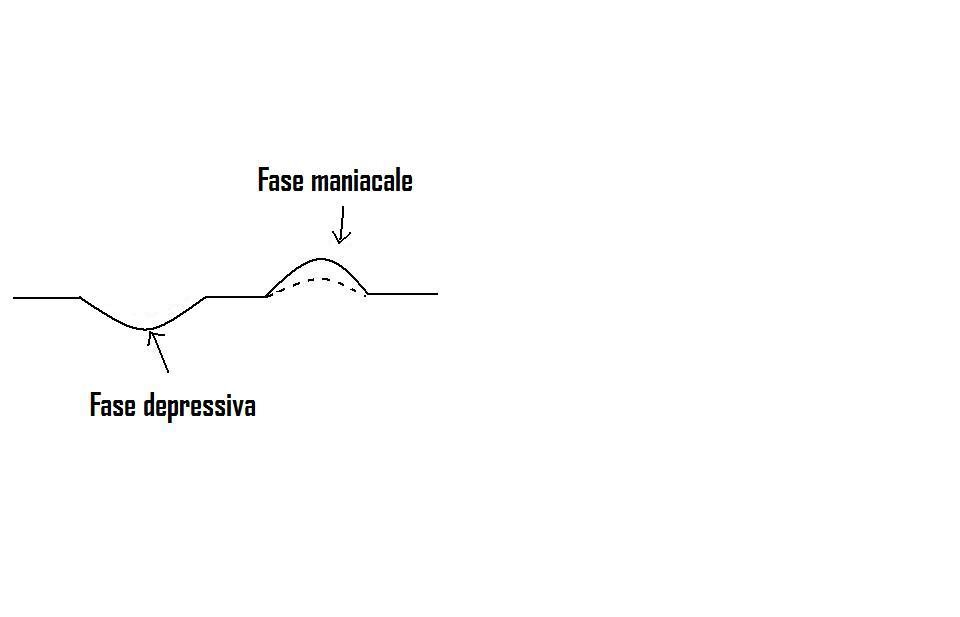
\includegraphics[width=0.9\textwidth]{02/image1.jpeg}
\end{figure}

Posto
che l'umore abbia un tono basale, si possono avere fasi di malattia sul
versante depressivo e fasi di malattia sul versante maniacale oppure
sono fasi depressive o solo fasi maniacali.

\paragraph{DEPRESSIONE MAGGIORE RICORRENTE} vuol dire che quel soggetto ha
solo manifestazioni depressive, è un paziente che non scivola dalla
parte opposta come nel caso del disturbo bipolare. Quindi se io avessi
un episodio depressivo questo potrebbe essere una manifestazione
iniziale di una depressione maggiore ricorrente o la prima
manifestazione di un disturbo bipolare, in questo caso però ho bisogno
di una fase maniacale e fino a quando non ce l'ho non posso fare
diagnosi di disturbo bipolare anche se questa possibilità è presente.
Pensate che si considera che circa il 15-20\% di quei soggetti che fino
a quel momento sono dei depressi maggiori ricorrenti possono diventare
dei pazienti con disturbo bipolare perché si manifesterà un episodio
maniacale.

Questo tipo di disturbo (depressione maggiore ricorrente) viene anche
definito \textbf{DEPRESSIONE UNIPOLARE}, perché le fasi di malattia sono
sempre e solo depressive: l'alterazione dell'umore è solo in questo
senso.

Si devono considerare alcune \textbf{caratteristiche,} per definire il
quadro di DEPRESSIONE MAGGIORE RICORRENTE (in cui la sintomatologia che
abbiamo visto si ripresenta più volte)\textbf{:}

\begin{itemize}
\item[1.]
  \textbf{il numero di episodi} Prendendo una popolazione di soggetti
  depressi il VALORE MEDIANO degli episodi è di 4: il 50\% dei soggetti
  ha da 1 a 4 episodi nella vita e il restante 50\% ha più di 4 episodi
  nella vita. È possibile ci siano pz con fasi numericamente limitate e
  altri con fasi frequenti.
\item[2.]
  \textbf{la durata degli episodi} è variabile. Valutando nella
  popolazione dei depressi la durata, la mediana è di 6 MESI: nel 50\%
  dei pz la depressione dura da almeno (due settimane per definizione) 6
  mesi, nell'altro 50\% dura più di 6 mesi , anche per alcuni anni!
\end{itemize}

\emph{NB: la media è diversa dalla mediana: in quest'ultima si considera
il valore che divide esattamente in due metà numericamente uguali il
campione (quindi non è influenzata dai valori estremi).}

\begin{itemize}
\item[1.]
  bisogna considerare il \textbf{rischio di suicidio} (10\% dei pz tenta
  e riesce) e il rischio aumenta in relazione a: familiarità, delirio,
  maggiore durata episodi e ripetuti fallimenti terapeutici.
\item[2.]
  \textbf{Insorgenza}: depressione ricorrente più facilmente compare
  dopo i 30 anni
\end{itemize}

\paragraph{CRITERI DELLA DEPRESSIONE MAGGIORE:}

Attualmente in Psichiatria vengono usati due sistemi diagnostici :

\begin{itemize}
\item
  \emph{\emph{L'International Classification of Diseases dell'OMS:}} si
  usa abitualmente ed è anche utilizzato per fare diagnosi di
  dimissione.
\item
  L'altro è quello \emph{\emph{dell'American Psychiatric Association}}
  (quinta ed ultima edizione nel 2013): ha avuto un grande e inaspettato
  successo. Quest ultimo è un manuale semplice che presenta vari sintomi
  i quali, se soddisfatti, permettono di arrivare ad un'indicazione
  diagnostica. Tuttavia è molto limitativo in quanto un sintomo ha lo
  stesso valore sia che sia legato alla depressione sia che sia legato
  ad altre patologie perché non indaga sul vissuto del paziente e quindi
  non ci permette di poter differenziare i vari casi.
\end{itemize}

Esempio: ``non uscire di casa'' perchè non si sente il desiderio/
piacere di uscire o perché si teme che fuori capiti qualcosa (stesso
sintomo ma diverse situazione). Come l'animale che ferito torna nella
tana cosi l' inclinazione di tutti quelli che stanno male è di ritararsi
e non stare in mezzo agli altri, non solo perchè sono infastiditi dalla
gente, ma anche perché notano la differenza con gli altri.

Esempio : ``insonnia'' nel paziente depresso si ha insonnia perché
durante la notte si angoscia pensando di essere incapace di svolgere le
funzioni del giorno successivo . Diverso è invece il caso del paziente
che si sveglia perchè ha tanta energia in corpo e quindi freme
nell'attuare i suoi compiti.

Questo è stato un sistema messo a punto, più che per la pratica clinica,
per permettere a chi faceva ricerca di selezionare campioni di pazienti
che avessero lo stesso disturbo, perchè si avevano dei campioni
assolutamente disomogenei. Per cui il tentativo era di scegliere, almeno
per i disturbi sulla depressione maggiore, pazienti che sono simili. Poi
purtroppo se ne è fatto un cattivo uso perché oramai questo viene usato
nella pratica clinica, per la formazione degli studenti, formazione
degli specializzandi. La realtà è diversa e più complessa.

Bisogna quindi analizzare in modo empatico la situazione per comprendere
in maniera corretta il vissuto del paziente e far diagnosi. Questo è il
motivo per cui il manuale , seppur molto in uso , è riduttivo.

Di norma per diagnosticare la Depressione Maggiore: dobbiamo valutare:
1.SINTOMI, 2.DURATA, 3.IMPATTO:

\begin{itemize}
\item
  Devono essere \emph{\emph{presenti contemporaneamente almeno 5 di
  questi nove sintomi:}}
\begin{itemize}
\item[1.]
  \textbf{Umore depresso per la maggior parte del giorno, quasi ogni
  giorno};
\item[2.]
  \textbf{Marcata diminuzione di interesse o piacere per tutte o quasi
  tutte le attività normalmente svolte dal paziente};
\item[3.]
  \textbf{Significativa perdita o aumento di peso o dell'appetito};
\item[4.]
  \textbf{Insonnia o ipersonnia};
\item[5.]
  \textbf{Agitazione o rallentamento psicomotorio};
\item[6.]
  \textbf{Faticabilità o mancanza di energia};
\item[7.]
  \textbf{Sentimenti di autosvalutazione o di colpa inadeguati,
  inappropriati o eccessivi};
\item[8.]
  \textbf{Diminuita capacità di pensare o di concentrarsi o presenza
  di forti indecisioni};
\item[9.]
  \textbf{Pensieri ricorrenti di morte, ricorrente ideazione
  suicidaria o tentativo di suicidio}.
\end{itemize}

Di cui almeno uno deve essere: 
\begin{itemize}
\item[(1)]
l'umore depresso per la maggior parte del giorno o 
\item[(2)]
la perdita di interesse e piacere per quasi tutte le
attività.
\end{itemize}

È ovvio che si deve sempre tener presente che il sintomo non deve essere
spiegato da un'altra patologia (Ad esempio il tumore del pancreas o
l'assunzione di sostanze possono portare ad un'alterazione dell'umore).
Quindi, in altri termini, dobbiamo verificare se è un disturbo
\emph{``primario''} cioè non riconducibile ad altre patologie o
\emph{``secondario''} se invece è dovuto a particolari malattie.

\item
  Deve avere una \emph{\emph{durata di almeno due settimane}} (si parla
  disturbo cronico se superiore a due anni): 2 settimane era un criterio
  necessario per definire il tempo però, gli episodi depressivi sono ben
  lontani da questa durata. Si giustifica questa affermazione partendo
  da questo dato: ammettendo di essere tutti pazienti depressi, di avere
  avuto tutti un episodio depressivo che ha avuto una durata: quindi ha
  avuto un'insolvenza, ha avuto una risoluzione e ciascuno dei pazienti
  ha la sua durata di malattia. Si può fare la media ma più che la
  media, che è esattamente la somma diviso il numero complessivo dei
  pazienti, ci interessa la cosiddetta mediana perchè se si avesse tra
  di loro persone con durate di malattia lunghissima (6 anni) la media
  risentirebbe profondamente di quei 2/3 casi che hanno durate estreme.
  Allora per evitare questo si usa la mediana. Mediana vuol dire quel
  valore che divide il nostro campione in 2 parti numericamente uguali.
  Quindi se si calcola la mediana della durata dell'episodio depressivo,
  si hanno 6 mesi (non 2 settimane). Cosa vuol dire avere una mediana di
  6 mesi come durata di episodio depressivo? vuol dire che se i pazienti
  sono 100, il 50\% del campione ha una durata inferiore ai sei mesi (da
  2 a 6 mesi) ma l'altro 50\% ha una durata di episodi che va oltre i 6
  mesi: infatti tra i disturbi cosiddetti cronici vi è anche la
  depressione maggiore. Tra questi i pazienti che ne sono affetti hanno
  episodi che durano anche altre 2 anni. Quindi se qui 2 settimane è un
  criterio temporale minimo, la realtà o quello che avviene nella
  pratica è ben superiore a queste 2 settimane, quindi almeno circa 24
  settimane. Tenete quindi presente che parliamo di una condizione che
  ha una durata prolungata.
\item
  Deve determinare un \emph{\emph{cambiamento della qualità di vita del
  paziente.}}
\end{itemize}

In realtà la diagnosi non è è sempre così schematica, infatti si possono
avere anche dei quadri di 3 sintomi ma con una depressione gravissima o
quadri con 6 sintomi ma una depressione lieve.

Constatazione: spesso i pazienti depressi non si recano dallo
psichiatra, infatti se prendiamo come esempio un paziente con i sintomi
3 (perdita di peso) , 4 (insonnia) ,6 (faticabilità) il primo sospetto
ricadrà su una patologia tumorale ma, se dopo i dovuti esami, continuano
a mancare le cause organiche sarà necessario riprendere in
considerazione la diagnosi di depressione. Per identificare (screening)
un paziente depresso è sufficiente verificare la presenza di una delle
due prime manifestazioni (sintomo 1 o 2).

Infatti, ricordiamo che dei famosi cinque sintomi almeno uno deve essere
o il primo o il secondo.

Analizziamo i sintomi uno alla volta:
\begin{itemize}
\item[1)]
\emph{Umore triste}: abbiamo una flessibilità stabile dell'umore, ed
il paziente si sente inspiegabilmente triste, cupo, avvilito,
sfiduciato, arrivando nelle forme più avanzate ad essere pessimista,
svuotato, angosciato o anche disperato.
\item[2)]
\emph{Perdita di interesse} : il soggetto diviene insensibile agli
eventi esterni, non è più in grado di provare emozioni e di avvertire le
esperienze piacevoli, condizione nota come \textbf{anedonia.} Un esempio
è il paziente anziano che non esce più di casa e smette di andare al
circolo perchè ha perso la voglia / il piacere / l'interesse / il
divertimento nel farlo. Quello che prima lo spingeva ad andare era il
provare piacere in quell'attività, ora invece avendo perso l'interesse
preferisce restare a casa.

Se analizzati questi due punti permettono di evitare tanti accertamenti
e collegano la sintomatologia ad un quadro di tipo depressivo. La
probabilità che un quadro depressivo venga riconosciuto se il paziente
riferisce astenia , perdita di attenzione , perdita di peso e insonnia è
bassa; diventa alta invece se il paziente piange e ammette la
depressione. Uno studio di dieci anni fa, svoltosi negli Stati Uniti, su
un campione di 300 casi di pazienti affetti depressione maggiore,
dimostra che dal GP ne venivano diagnosticati correttamente solo l' 8\%.
Il trattamento una volta instaurato porta agli stessi esiti sia che il
paziente sia trattato dal medico di medicina generale o dallo
psichiatra. Il problema però è che il medico di medicina generale tende
a sottovalutare la probabilità che quel quadro sintomatologico sia
nell'ambito di un disturbo depressivo.

Importante ricordare che si può anche avere un quadro di depressione in
cui manca la tristezza; infatti è necessario solo uno dei due sintomi
quindi possiamo avere quadri di \emph{\textbf{depressione sine
depressione}:} l'elemento più evidente non è la tristezza ma la restante
sintomatologia.
\begin{itemize}
\item[3a)]
\emph{Inappetenza}: Il calo ponderale è un sintomo importantissmo. Il
paziente affermerà: `` il cibo non ha sapore'', ``mangio perchè so che
devo mangiare ma se seguissi la mia inclinazione non mangerei'', `` il
sapore è amaro''. Questo sintomo è collegato a una perdità del piacere
per cui il cibo non è più una fonte di gratificazione.
\item[3b)]
\emph{Aumento di peso:} in genere in 2/3 dei casi si manifesta
inappetenza , ma in 1/3 dei casi, paradossalmente, si ha un aumento di
peso legato alla tendenza a mangiare di più.
\end{itemize}

\begin{itemize}
\item[4a)]
\emph{Insonnia}: rappresenta uno dei sintomi più precoci e si
manifesta con ripetuti risvegli notturni (\emph{insonnia intermedia}) o,
nelle forme più gravi, con un risveglio precoce, alcune ore prima
dell'orario abituale (\emph{insonnia terminale}). Il sonno, in ogni
caso, non risulta ristoratore, poiché gravato da continui \emph{incubi}
e \emph{sensi di apprensione}. Sono soggetti che vanno a dormire,
riescono ad addormentarsi ma solo dopo poche ore si svegliano angosciati
all'idea delle azioni che dovranno svolgere quella giornata, si sentono
incapaci di svolgere la loro normale routine (che hanno sempre condotto)
e anche le azioni più semplici risultano difficili (un elettricista in
difficoltà a cambiare una lampadina, una casalinga incapace di mettere
la pentola a bollire sul gas) . Il paziente diventa disordinato, non
riesce a fare da mangiare, non riesce a fare nulla e prova un'angoscia
assoluta e senso di colpa che sembrano diminuire verso sera
semplicemente per il fatto che la giornata si è conclusa e non rimane
più nulla da fare.

\item[4b)]
\emph{Ipersonnia}:di solito gli stessi soggetti che mangiano di più
sono anche gli stessi che dormono per più tempo. Non è matematica come
cosa ma spesso è cosi.

Inoltre l'aumento di peso e ipersonnia sembrano collegati a delle forme
\emph{stagionali} cioè depressioni che in genere esordiscono verso
ottobre, quindi nei mesi autunnali, e si risolvono nei mesi primaverili
(simil letargo).
\end{itemize}

\item[5)]
\emph{Agitazione e rallentamento psicomotorio:}Durante un colloquio
vi possono essere pazienti che non riescono a stare seduti quindi si
alzano continuamente o camminano spesso oppure pazienti completamente
immobili, inespressivi e simili a delle statue.

Una caratteristica della depressione maggiore, o disturbo unipolare, è
la CATATONIA:le manifestazioni sono di una gravissima inibizione
psicomotoria, tanto che nelle forme più avanzate si può arrivare a delle
vere e proprie condizioni di arresto psicomotorio, il cosiddetto
``\textbf{stupor melancolicus}'', in cui il paziente rimane immobile a
letto, senza reagire agli stimoli esterni e senza nutrirsi, spesso
avendo anche un blocco della funzione vescicale ed intestinale. Se
proviamo a sollevargli un braccio sentiamo una resistenza che in modo
costante cede alla forza che io applico, a un certo punto se smettiamo
di applicare forza il braccio del paziente rimane sollevato come lo
abbiamo lasciato tant'è che veniva definito ``la flessibilità della
cera''.

E' più frequente trovare catatonie da disturbi dell'umore, soprattutto
bipolare, rispetto a disturbi schizofrenici catatonici.

\item[6)]
\emph{Astenia:} si stancano a svolgere anche le azioni più semplici,
non riescono a condurre la loro normale routine.

\item[7)]
\emph{Sentimenti di colpa e svalutanti}: si sentono incapaci di
svolgere le azioni più semplici e per questo provano un forte senso di
colpa.

È noto che a volte i pazienti depressi sono talmente inibiti che non
riescono neanche a suicidarsi.Questo è vero, succede che il paziente è
talmente inibito che addirittura non riesce neanche a piangere. Questo
si riferisce soprattutto al discorso dell'inibizione, più che altro
motoria,per cui io non riesco neanche a lanciarmi dalla finestra e
neanche ad alzarmi per fare questo.

\item[8)]
\emph{Ridotta capacità di concentrazione o di pensiero}: Le funzioni
cognitive sono alterate, con un marcato rallentamento dell'attività del
pensiero ed una condizione di ottundimento e di mancanza di chiarezza,
spesso associata ad una sensazione di ``avere la testa vuota''; i
contenuti del pensiero, pochi, sono dolorosamente cristallizzati su
pochi argomenti a contenuto melanconico, su cui il paziente ritorna
costantemente (\textbf{ruminazioni mentali} o \textbf{idee coatte}), ed
anche la memoria è intaccata, sia negli aspetti di rievocazione che di
fissazione, tanto che in alcuni pazienti si possono raggiungere delle
condizioni simili a quella della demenza senile. Infatti in passato si
associavano alcuni stati del paziente depresso alla demenza ma con una
possibile regressione. Dal momento che la regressione nella demenza vera
e propria è impossibile è stato coniato il termine di
\textbf{\emph{pseudo demenza}.}

Nel quadro di tipo depressivo il paziente afferma: `` io provo a leggere
ma non c'è verso che mi entri in testa qualcosa''. Tutti questi pazienti
riferiscono infatti oltre alla mancanza di piacere nel fare le cose
anche la mancanza di concentrazione e di attenzione.

I pazienti dementi diversamente con tono non angosciato minimizzano la
situazione cercando di colmare la loro incapacità legata a funzioni
cognitive compromesse. Nei depressi durante i test cognitivi
all'aumentare del tempo o della difficoltà si nota una diminuzione del
risultato dato che non riescono a mantenere la concentrazione. I
pazienti dementi invece cercano in tutti i modi di farcela ( Esempio: il
soggetto demente chiede la data prima del giro visite per non mostrarsi
impreparato quando gli sarà chiesta dal medico). Infine il paziente
depresso non sbaglia mai, il demente invece spesso sbaglia stanza e
compie azioni sconnesse.

\item[9)]
\emph{Pensiero ricorrente di morte, di suicidio}:

\textbf{\emph{Depressione vitale}} : particolare umore che il soggetto
coglie come uno stato d'animo che non ha mai avuto, che lo pervade e che
lo distacca completamente dalla realtà. Non c'è nulla che lo possa
modificare. Si trova in genere associato al \emph{sentimento della
mancanza di sentimento:} '', un angoscioso senso di non provare più
alcunché per le persone o le cose prime care (``\emph{io non provo più
nulla'')}. Un esempio può essere una neomamma che, pur riconoscendo di
avere desiderato con tutta se stessa la figlia, afferma di non provare
nessun sentimento nei sui confronti, a fatica sa che è sua figlia e non
riesce neanche a tenerla in braccio. Questa mancanza di sentimento viene
percepita con un angoscia estrema perché si ritengono cattive madri.

Fondamentale è poi la comprensione di come questi pazienti vivano il
\emph{tempo interiore}, poiché nell'episodio depressivo vi è uno
\textbf{scollamento del tempo cronologico dal tempo interno}: per il
paziente depresso le giornate appaiono interminabili, le ore non
scorrono mai, ed i giorni, i mesi e gli anni a venire sono tutti visti
in chiave negativa, come un tempo di sofferenza infinita da cui spesso
traggono origine le \emph{idee suicidarie}. Quindi \emph{il tempo} in
questi pazienti viene vissuto in un modo particolare: si capisce che il
soggetto si trova in questa condizione di malessere \emph{presente} e
che spesso ripercorre il \emph{passato} vivendolo però con il malessere
emotivo del momento. In altri termini: è come se il passato incombesse
sul presente e nello stesso tempo è come se il presente si fosse
dilatato inglobando nel vissuto anche il passato. Il problema però non è
tanto il passato ma ciò che preoccupa maggiormente il paziente è il
\emph{futuro}.

Per meglio capire il concetto riporto questo esempio: un soggetto di 32
anni ha più o meno una aspettativa di vita di 82-83 anni, quindi sa
potrà vivere per altri 50 anni ma il problema è: come li vivrò? Non vede
soluzione per il suo malessere presente, non vede via di uscita dalla
sua condizione, il presente ingloba anche il futuro. Questa situazione
crea un'angoscia tale per cui, piuttosto che vivere altri 50 anni in
questa sofferenza atroce, preferiscono ``anticipare la data'' vedendo
nel suicidio l'unica via per porre fine al loro dolore.
\end{itemize}

\begin{itemize}
\item
\emph{Esempio1} : Alcuni anni fa in Valle d'Aosta dei turisti, facendo
una passeggiata in un sentiero che fiancheggiava un laghetto, si
accorsero che nel laghetto c'era una donna con due bambini. La madre
raggiunta dai soccoritori disse ``lasciatemi stare , lasciatemi morire
``. Non vedeva soluzione alla sua sofferenza se non la morte. Bisogna
però capire perché ha conivolto nel suo suicidio anche i figli: la madre
era convita che la sua sorte sarebbe toccata anche ai suoi figli per cui
portandoli con sè avrebbe risparmiato loro una vita di sofferenze. (Il
\emph{canto notturno di un Pastore errante dell' Asia} di Leopardi
finisce con : `'è funesto a chi nasce il dì natale'' questa frase per il
depresso è \emph{letterale}.)

Spesso in questi casi si parla di \textbf{\emph{suicidio altruistico}}
perché il paziente è convinto di risparmiare alle persone a cui vuole
bene una vita di sofferenza estrema .

\item \emph{Esempio 2}: 7-8 anni fa a Reggio Emilia un padre uccise il figlio
di 3 anni, la moglie, la vicina di casa che li ospitava gratuitamente e
poi tentò il suicidio ma non riuscì nell'intento di togliersi la vita.
Alla domanda dello psichiatra riguardo il perchè di queste azioni,
affermò: ``l'ho fatto per il troppo amore''. Nell'ottica del paziente
depresso ha risparmiato loro degli anni di sofferenza \emph{suicidio
allargato di tipo depressivo} (Da non confondere con il marito che
uccide la moglie per gelosia che affermerebbe ``Lei o sta con me o non
sta con nessuno'' e non `` l'ho fatto per risparmiarle anni ed anni di
sofferenza'').

\item \emph{Esempio 3}: alcuni pazienti affermano : ``la ringrazio dottore per
quello che fa, ma per me non c'è nulla da fare. Mi salva e io starò
altri 50 anni cosi ? ..mi lasci morire perchè per me non c'è nulla da
fare''.

\item \emph{Esempio 4}: Conclusione: Data tale definizione si dimostra come
nessun paziente con depressione possa comportarsi allo stesso modo del
pilota dell'Airbus Germanwings. Il pilota infatti:

\begin{itemize}
\item
  ha pianificato tutte le sue mosse, un paziente depresso non è capace
  di pianificare ma anzi si sente spesso un incapace.
\item
  Il depresso non è un omidicia, ma un suicida. Può coinvolgere altri ma
  saranno persone da lui molto amate a cui vuole risparmiare il dolore
  che lui sta provando (suicidio altruistico).
\end{itemize}
\end{itemize}

L'episodio depressivo può inoltre caratterizzarsi per la presenza di
\textbf{MANIFESTAZIONI DELIRANTI} (Delirio: dal latino, esco dal solco.
Il solco è il giudizio che ciascuno di noi ha della realtà e è ciò che
appare immediatamente e fa parte del senso comune. L'alterazione nasce e
si genera dall'alterazione dell'umore) , e in questo caso si parla di
\emph{deliri affettivi} o \emph{olotimici}, che possono essere
essenzialmente di 3 tipi:

\begin{itemize}
\item[1.]
  DELIRIO di ROVINA (ECONOMICA): (il paziente crede che, a causa della
  sua condizione attuale, non sarà più in grado di sostenere
  economicamente la sua famiglia, per cui crede di essere sul lastrico
  anche se in realtà è ricco).
\item[2.]
  DELIRIO di COLPA: (il paziente vede la sua condizione di sofferenza
  attuale come la punizione di una colpa compiuta in passato, spesso del
  tutto sproporzionata alla condizione attuale).
\item[3.]
  DELIRIO SOMATICO: (il paziente è convinto di avere una malattia
  incurabile, spesso identificata come causa del suo male, ma crede che
  gli altri vogliano tenerglielo nascosto).
\end{itemize}

Questi tre tipi di deliri possono poi associarsi tra loro costituendo
delle forme particolarmente gravi:

\begin{itemize}
\item
  come il \textbf{\emph{delirio nichilistico}}, in cui il paziente è
  convinto di non avere più una famiglia o addirittura parti del corpo,
  arrivando persino a negare la propria esistenza,
\item
  alla cosiddetta \textbf{\emph{sindrome di Cotard}}, in cui il paziente
  crede di essere morto e dannato a permanere sulla terra per l'eternità
  ad espiare le sue colpe oppure crede di essere l'unico uomo rimasto in
  vita, ma mentre lui soffre sulla terra, tutti gli altri sono in
  paradiso.
\item
  Nelle fasi avanzate non è poi raro riscontrare altre forme di delirio,
  che sono incongrue con l'umore, come il delirio di gelosia (piuttosto
  comune in verità), il delirio di persecuzione, di veneficio, di
  inserzione o furto del pensiero.
\end{itemize}

Queste forme di delirio possono essere OLOTIMICHE (congruenti all'umore)
o NON OLOTIMICHE.

Analizziamo le varie tipologie di delirio riferendoci a particolari casi
clinici:

\begin{itemize}
\item[1.]
  \textbf{\emph{DELIRIO DI ROVINA:}}

Vediamo cosa si intende con esempio:

\emph{Caso clinico}:

Il paziente è un avvocato che è diventato incapace di svolgere il suo
lavoro che ha sempre fatto: afferma di rimanere fermo davanti alle
pratiche e di non riuscire ad andare avanti nella lettura (era un
esordio di depressione). Il problema però non si è limitato a questo:
egli nei giorni seguenti ha cominciato a maturare la convinzione che,
non riuscendo più a fare il suo lavoro, avrebbe perso i clienti e con
questo i soldi e il lavoro con cui manteneva la famiglia. La moglie, di
fronte a questi discorsi fatti dal marito, ha cercato di convincerlo
della mancanza del problema con un dato di fatto: i conti in banca, che
dimostravano che la famiglia non sarebbe comunque andata verso problemi
economici. Tuttavia il pz continua ad insistere. In una delle visite il
pz chiede di parlare senza la moglie presente, dovendo dire una cosa che
sarebbe stata per lei spiacevole: egli era andato in autostrada per
cercare un punto da cui buttarsi. L'avvocato viene trattato (era al 3\textsuperscript{o}
episodio di malattia), guarisce e torna a condurre normalmente la sua
vita fino a quando dopo circa 3 anni una delle sue segretarie lo trova
morto in studio sulla sua scrivania: si era sparato.

\emph{Cos'è successo?} Risolto il precedente episodio di depressione
dopo tre anni aveva avuto una ricaduta. Ripartendo con la stessa
convinzione (ora delirante) di essere la causa della rovina economia sua
e della sua famiglia (si parla di DELIRIO DI ROVINA), si è tolto la
vita.

Consideriamo due aspetti del DELIRIO DI ROVINA:

\begin{itemize}
\item
  Questo delirio viene definito \emph{OLOTIMICO} dalla psichiatria
  classica e delirio CONGRUO ALL'UMORE dalla visione più moderna: se si
  ricostruisce l'esperienza delirante possiamo comprendere questa solo
  sulla base della depressione. Ovvero la depressione aveva causato in
  lui disturbi cognitivi (concentrazione, attenzione), difficoltà a
  raggiungere obiettivi, stanchezza\ldots{} e tutto questo ha generato
  (appunto sulla base della depressione), l'impossibilità di mantenere
  una attività lavorativa e quindi da questo si è sviluppato il delirio
  di rovina. È stato quindi, classicamente, definito ``OLOTIMICO''
  perché è l'alterazione dell'umore che fa da terreno per lo sviluppo
  dell'esperienza delirante stessa delirio \emph{congruo con l'umore}
  appunto perché è insito e nasce dall'esperienza depressiva. Ripetendo
  con altre parole: Il Delirio olotimico è connesso strettamente con
  l'alterazione dell'umore che ci permette di comprendere in termini di
  determinismo come mai il soggetto è arrivato a sconvolgere la realtà.
\item
  Il pz non si suicida al 3\textsuperscript{o} episodio di malattia grazie al trattamento
  ma si suicida al 4\textsuperscript{o} episodio: come è possibile che il pz, pur avendo
  avuto già degli episodi depressivi che si erano risolti, non sia
  riuscito a rendersi conto e a realizzare che si sarebbe ripreso anche
  da questo episodio? Scatta un altro meccanismo: il pz si rende conto
  dell'episodio depressivo (stessi sintomi dei precedenti), ma in questo
  egli non ha più la speranza, si convince del fatto che gli altri
  episodi non fossero come questo (in realtà l'episiodio è uguale ai
  precedenti) e che non ci sia più futuro o possibilità di cambiare la
  situazione attuale. Questo fa sì che le idee suicide, presenti anche
  negli episodi precedenti, siano portate a compimento. Dal punto di
  vista del pz l'episodio è diverso e non è possibile uscirne, non c'è
  futuro.
\end{itemize}

\item
  \textbf{\emph{IL DELIRIO DI COLPA:}}

Le ragioni della colpevolezza possono essere le più svariate, sia per
gesti fatti che per quelli non fatti.

\emph{Caso clinico 1:}

Il paziente è una donna che ha appena partorito. Guardando la storia
clinica della paziente apprendiamo che intorno al 7\textsuperscript{o} mese la pz si era
presentata al PS chiedendo di partorire nella totale convinzione che il
figlio stesse male. Viene fatta una visita ginecologica, tutto risulta
nella norma, la pz viene rassicurata e mandata a casa. Il giorno dopo di
nuovo si presenta e di nuovo vengono fatti accertamenti: non c'è niente
di irregolare, quindi il ginecologo decide di chiamare uno psichiatra
per la pz, ma questa non accetta e va a casa. Non si sa più nulla fino a
dopo il momento del parto in cui alla visita pischiatrica afferma:
\emph{``avete già dato in adozione mio figlio?''.} Viene indicato il
ricovero, la pz accetta.

Perché la pz ha detto questa frase?

Il problema è che la pz non si sente adeguata, è convinta di non potere
essere una buona madre. Vediamo l'estrema conseguenza di questi pensieri
e di questo stato d'animo, infatti la pz vive la gestazione pensando di
essere tanto incapace che anche il suo corpo non sia adeguato allo
sviluppo del bambino: il suo utero era inadeguato per il figlio, non era
lui malato ma lei che lo poteva far ammalare.

\emph{Caso clinico 2}: una pz che in episodio depressivo si è
colpevolizzata per aver preso alcuni sassi da un torrente durante una
passeggiata.

\item[3.]
  \textbf{\emph{IL DELIRIO DI PERSECUZIONE:}}

\emph{Non è olotimico}, a meno che non ci sia effettivamente la
possibilità di identificare una causa alla base (effettivamente il pz ha
commesso un atto che ``giustifica'' questi pensieri, che ci permette di
distinguere il deliro di colpa dal delirio di persecuzione propriamente
detto).

\emph{Caso clinico:}

Ragazzo di 23 anni ricoverato per episodio depressivo. Egli era orfano e
viveva con il fratello. Qualche mese prima dell'esordio depressivo erano
accaduti una serire di eventi: il fratello, avendolo visto fumare
marjuana lo aveva ammonito a smettere o avrebbe allontanato da casa; la
fidanzata, sempre per la stessa ragione, aveva minacciato di lasciarlo;
il datore di lavoro, dato il suo comportamento poco responsabile al
lavoro, aveva minacciato il licenziamento. Mentre era ricoverato, una
notte è stato trovato intento a tagliarsi i polsi con la lametta del
rasoio. Quale è stata la ragione di questo suo gesto? Egli ha riferito
di avere sentito le sirene dei carabinieri che lo sarebbero venuto a
prendere (notate che in realtà erano le sirene della ambulanze della
croce rossa, lì a fianco), processare, condannare e imprigionare per
quello che aveva fatto (quindi si sarebbe ammazzato piuttosto).

\textbf{Come facciamo a discriminare se in questo caso si tratta di
delirio di colpa o di delirio di persecuzione?} È stato chiesto al pz se
avesse fatto qualcosa che giustificasse tutto ciò ed egli ha riferito
quello che aveva fatto (e che giustifica il DELIRIO DI COLPA, ``è giusto
che io sia giustiziato per quello che ho fatto''). \emph{Invece nel
delirio di persecuzione i soggetti dicono di non sapere perché la
Giustizia se la prenda con loro}.

\item[4.]
  \textbf{\emph{IL DELIRIO SOMATICO}}:

Il delirio somatico può essere:

\begin{itemize}
\item
  riferito al pz
\item
  riferito ai famigliari (ad es una donna che si era convinta del fatto
  che il figlio avesse la leucemia\ldots{})
\end{itemize}

Quindi a volte il vissuto somatico è talmente alterato dagli episodi
depressivi che ciò che riferiscono i pz ha le caratteritiche del
delirio. Lo si riscontra soprattutto nell'anziano, quando il corpo
invecchia e il soggetto si rende conto di questi problemi.

Per capire di cosa si tratta si vedano questi esempi:

\emph{Caso clinico 1:}

Marito e moglie, circa 60 anni. Il marito esce di casa e quando torna
trova la moglie in piedi davanti al lavello con i polsi tagliati
profondamente (arteria e tendini) \emph{notate che caratteristicamente
in questi casi il pz prepara stracci e sta sul lavello per non
sporcare}. Il marito riferisce di non essersi accorto di nulla, non
trova spiegazione.

Viene poi ricostruita la storia con la pz: aveva avuto una crisi
epilettica qualche mese prima, non si è scoperta la causa (non aveva
tumori, nulla..), ma le si era insinuato il dubbio di avere un tumore e
che gli altri non volessero dirglielo: si convince di avere pochi mesi
di vita e decide di suicidarsi piuttosto che arrivare allo stadio
terminale della malattia.

\emph{Caso clinico 2:}

Pz depressa che è convinta di avere una fistola tra l'esofago e la
trachea perché avverte un odore di putrefazione, causato dal cibo che
passa in trachea a causa della fistola e si deposita nelle basi
polmonari dove va in putrefazione.

\emph{Domanda studente: l'ipocondria fa parte del delirio somatico?}

Generalmente il vissuto somatico del depresso è tutto alterato: è un pz
che dimagrisce, è deperito, etc, quindi il medico potrebbe pensare che
abbia di tumore e anche il pz si convince di ciò\ldots{}poi si arriva
fino al vero e proprio delirio.
\end{itemize}

\paragraph{EZIOPATOGENESI DELLA DEPRESSIONE MAGGIORE:}

\begin{figure}[!ht]
\centering
	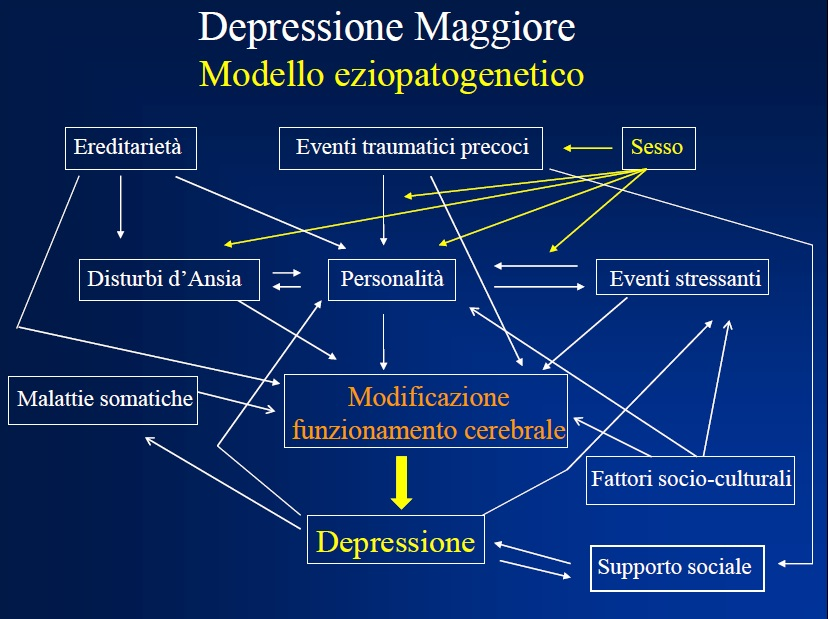
\includegraphics[width=0.9\textwidth]{02/image2.jpeg}
\end{figure}

Come non esiste un esame che ci permetta di fare diagnosi così non ho
nemmeno un'idea precisa sulle cause, ma sappiamo che esistono per
ciascun disturbo dei fattori di rischio.

La stragrande maggioranza dei disturbi psichiatrici non hanno
un'eziologia unica: \textbf{ci muoviamo nell'ambito dell'eziologia
multifattoriale}.

Cosa intendiamo per rischio? Utilizziamo una metafora.

Nel momento in cui noi siamo stati concepiti ci è stato consegnato un
recipiente, un'anfora che può avere o non avere una determinata quantità
di liquido dentro; il liquido rappresenta i fattori di rischio. Tanti
più fattori di rischio ho, tanto è più probabile che il livello del
liquido si avvicini al colmo dell'anfora e travasi. Fintantoché ho solo
liquido e non tracima, io rimango nell'ambito della vulnerabilità, del
rischio, ma non ho la malattia; quando tracima passo dal rischio alla
malattia.

I fattori di rischio possono non essere presenti sempre in un dato
momento ma si possono aggiungere in fasi successive: ne posso avere al
momento della nascita, se ne possono aggiungere nei primi anni di vita,
durante l'adolescenza e anche in età adulta. Più se ne aggiungono più è
probabile che la mia anfora tracimi. Se non tracima non mi ammalo, però
attenzione perché quel rischio io lo trasferisco e lo consegno ai miei
figli, una sorta di eredità.

I rettangoli nella slide sono tutti fattori di rischio conosciuti;
esistono alcuni fattori protettivi: come il supporto sociale che mi
``tolgono liquido''. Questi fattori di rischio sono interconnessi, si
influenzano.

Vari studi hanno ormai messo in luce con chiarezza che si tratta di un
\textbf{\emph{processo eziopatogenetico complesso}}, in cui rientrano
sicuramente delle componenti di \emph{ereditarietà}, che predispongono
allo sviluppo del disturbo dell'umore, ma su cui vanno poi ad agire
anche altri fattori, quali il \emph{sesso}, gli eventuali \emph{eventi
traumatici precoci}, lo \emph{stress}, i \emph{fattori socio-economici e
culturali}, le \emph{malattie somatiche} e la \emph{personalità} del
paziente stesso.

\subparagraph{EREDITARIETA'}

Prendiamo in esame una serie di studi che ci permettono di analizzare il
contributo genetico nei confronti della depressione maggiore (modello
adattabile anche a tutti gli altri disturbi psichiatrici in generale).

\begin{itemize}
\item[1.]
  Intervista strutturata a \textbf{100 persone prese a caso} che
  dovrebbero rappresentare la popolazione generale per verificare quanti
  di questi sono stati affetti da depressione maggiore nell'ultimo anno.
  Il dato va dal 4\% dei maschi al 9\% delle femmine con valori
  intermedi attorno al 6\%
\item[2.]
  Cambio popolazione\textbf{: 100 famigliari di primo grado} di un
  paziente affetto da depressione maggiore. La percentuale di quanti ne
  sono affetti è decisamente più alta rispetto alla popolazione
  generale, il che vuol dire che in quella famiglia c'è qualcosa che
  predispone i suoi componenti alla depressione maggiore. Si è dibattuto
  per anni su questo: se fosse più la genetica o l'ambiente ad influire.
\item[3.]
  Studio sulle coppie di \textbf{gemelli}: confronto circa la
  \emph{concordanza} tra gemelli omozigoti ed eterozigoti; cioè ammalato
  uno qual' è la probabilità che sia ammalato anche l'altro. L'idea di
  fondo è che, se si tratta di una malattia con base genetica rilevante,
  mi aspetto che la concordanza tra fratelli omozigoti (DNA identico)
  sia molto più alta rispetto alle coppie di fratelli eterozigoti.
  Questo è stato confermato. Emerge però un dato: la concordanza non è
  del 100\% sappiamo quindi che la genetica ha un ruolo, ma non ci
  spiega perché quel soggetto è malato; inoltre non posso sapere se
  questi due gemelli che vivono con una madre depressa non siano stati
  influenzati maggiormente da questo fattore ambientale?
\item[4.]
  Studio condotto sui \textbf{figli adottivi}. Sono messi a confronto
  due gruppi di bambini adottati da famiglie senza disturbi; la
  differenza tra i due campioni sono i genitori biologici: quelli di un
  gruppo presentano madre o padre o entrambi affetti da depressione,
  quelli dell'altro no. L'unica differenza quindi è la dotazione di
  base, vulnerabilità per la malattia di un gruppo ricevuta dai
  genitori. L' idea è che in questo modo si possa valutare se abbia un
  peso maggiore la vulnerabilità genetica famigliare o l'ambiente. Nel
  primo caso analizzando i bambini da grandi dovrei riscontrare una
  percentuale maggiore di malati di depressione nel gruppo di individui
  vulnerabili; nel secondo caso qualora l'ambiente famigliare riesca ad
  annullare la vulnerabilità avrei un pareggio e, quindi, percentuali
  vicine a quelle della popolazione generale. Vince la vulnerabilità.
\end{itemize}

\begin{figure}[!ht]
\centering
	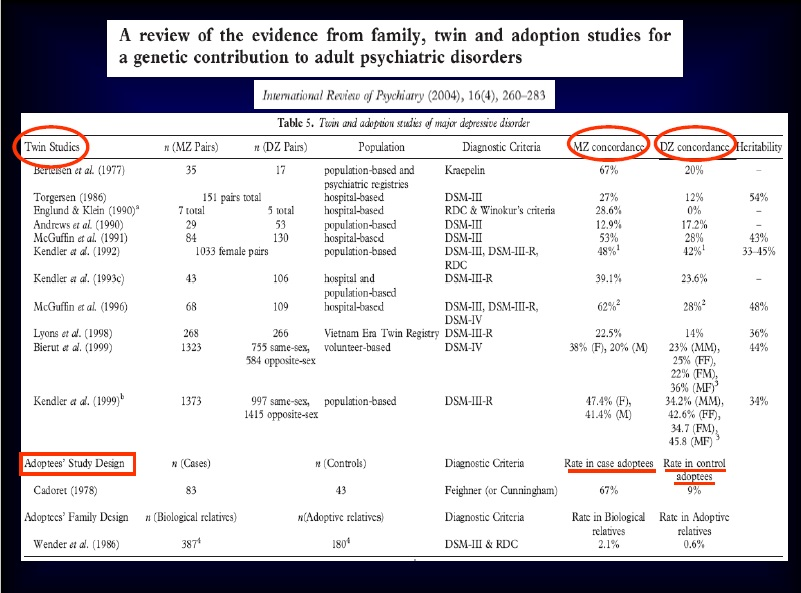
\includegraphics[width=0.9\textwidth]{02/image3.jpeg}
\end{figure}

Quello che emerge è che l'ereditarietà è uno dei fattori che dobbiamo
considerare attentamente. Non è detto, tornando alla metafora, che la
quantità di liquido sia uguale per tutti in termini di rischio genetico:
pensiamo ad esempio ad un figlio concepito da una coppia in cui uno dei
due genitori sia \textbf{bipolare}, la sua anfora è già piena per il
70\%; cosa analoga per la \textbf{schizofrenia}. L'influenza è molto
meno marcata per la \textbf{depressione maggiore} e i \textbf{disturbi
d'ansia}.

In realtà la situazione è più complessa: all'interno della schizofrenia
ad esempio non è detto che tutti ricadano nella stessa percentuale di
rischio genetico. Ciò si può osservare direttamente sui pazienti: padre
schizofrenico con 4 figli, tutti e 4 malati di schizofrenia, padre
schizofrenico con due figli gemelli eterozigoti che si sono ammalati a
distanza di 15 giorni uno dall'altro ed è chiaro che in questi due casi
il peso della genetica sia determinante; in altri casi invece no, ad
esempio tre figli di cui uno solo si ammala (vedi figlio di Gianni
Agnelli che si è buttato da un ponte). La penetranza di questo che non
sappiamo tutt'oggi che gene sia, su quale cromosoma, è variabile tanto
da determinare in alcuni casi un impatto devastante in altri molto meno.
Questo è un problema che viene sollevato dagli stessi pazienti nel caso
in cui, ad esempio vogliano un figlio e vi chiedano ``diventerà
esattamente come me?''. Quella che dobbiamo fornire è un'informazione
corretta riguardo l'accertato fattore di rischio, sulla base della quale
possano decidere liberamente.

\subparagraph{SESSO}

\begin{figure}[!ht]
\centering
	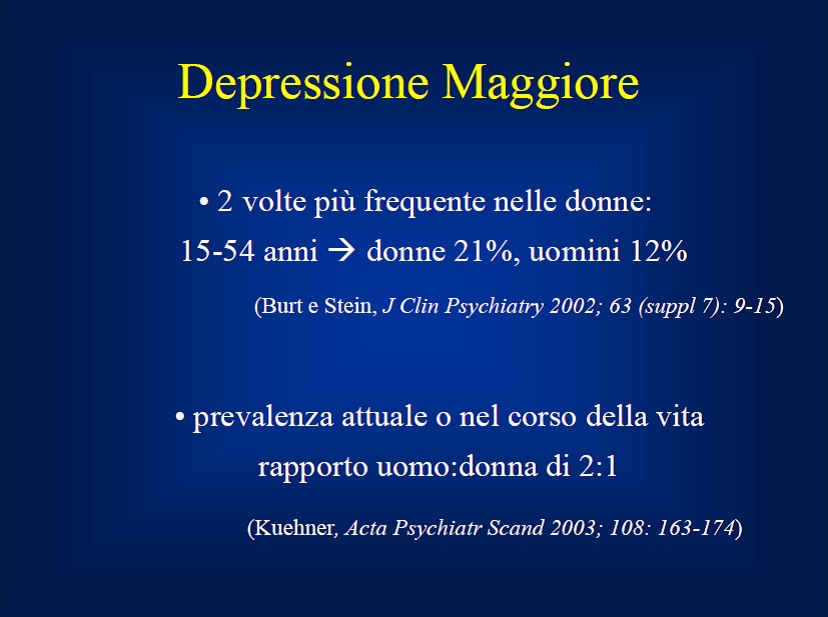
\includegraphics[width=0.9\textwidth]{02/image4.jpeg}
\end{figure}

Tra i 15 e i 54 anni il 21\% (quindi 1 donna su 5) soffrirà di un
episodio depressivo maggiore, contro il 12\% (quindi la metà, 1 su 10
degli uomini). Questo vale per tutta la vita.

Si sono effettuati degli studi sui bambini con grande difficoltà, dovuta
al fatto di studiare la depressione su un bambino che non dice mai
``sono triste'' e quindi bisogna prestare attenzione al suo
comportamento: contatto con gli altri, loquacità, ecc. La cosa
interessante emersa è che l'incidenza tra i bambini tende ad essere
simile indipendentemente dal sesso. Questo fino ai 14 anni circa, ovvero
l'età del menarca in cui questa differenza compare e si mantiene: in
qualche modo \textbf{gli ormoni sessuali sono implicati}.

Studio in cui si è andato a valutare l'effetto di un trauma micidiale
come la violenza sessuale nei bambini e qual era l'effetto di questo
trauma per la vita adulta

\begin{figure}[!ht]
\centering
	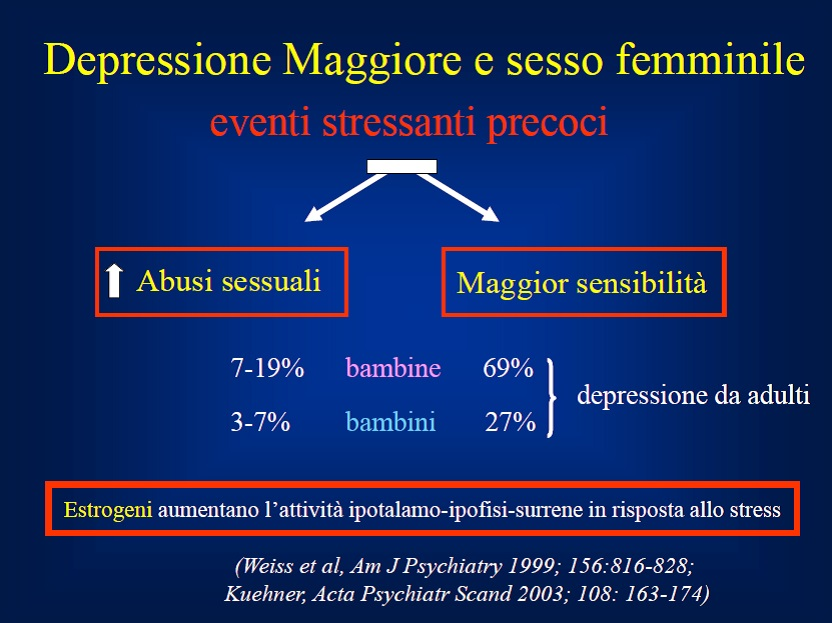
\includegraphics[width=0.9\textwidth]{02/image5.jpeg}
\end{figure}

Risulta rilevante come i 2/3 delle femmine abusate abbia sviluppato un
episodio depressivo contro 1/3 dei maschi, quindi a parità di gravità
dell'evento traumatico le femmine sembrano essere meno resistenti. La
spiegazione chiama in causa il nostro sistema di risposta ad un insulto
esterno, stress: \textbf{l'asse ipotalamo ipofisi surrene} che va visto
come un sistema che permette di affrontare i cambiamenti. Il problema è
che questo sistema viene sensibilizzato dalla presenza degli estrogeni,
il che vuol dire che, a parità di stimolo, l'attivazione è molto
maggiore se ci sono estrogeni e analogamente a parità di risposta basta
uno stimolo minore. Il ``burattinaio'' implicato sarebbe il CRF
(corticotropin-releasing factor) e ciò è interessante per due motivi.

\begin{itemize}
\item[1.]
  Iniettando questa proteina nella scimmia osservo una cosa molto
  interessante, ovvero che l'animale non sta più con gli altri, non si
  alimenta più come prima, non esplora più il territorio, non si
  accudisce come prima e se ha dei piccoli li trascura, il che pur
  parlando di una scimmia ci ricorda aspetti del malato di depressione
  maggiore. Sono stati studiati dei farmaci antidepressivi capaci di
  bloccare l'effetto del CRF, supportati anche dal fatto che nelle forme
  più gravi di depressione si sono dosati dei livelli di cortisolo
  abnormemente elevati , con perdita ritmo circadiano giorno-notte.
\item[2.]
  Questo sistema è quello che ci fa ricordare i traumi e tra gli eventi
  che possono far tracimare l'anfora contenente i fattori di rischio ci
  sono proprio questi scossoni, eventi traumatici. Sistema che si attiva
  immediatamente ed è il momento in cui è molto più facile che l'anfora
  si rovesci, rendendosi manifesta la malattia. Molto probabilmente
  questo sistema si è sviluppato in tal modo a fini evolutivi: è la
  femmina ad avere le prole e necessita di reazioni molto più rapide
  agli stimoli esterni per proteggere la prole.
  \end{itemize}
  
\subparagraph{EVENTI TRAUMATICI PRECOCI}

\begin{figure}[!ht]
\centering
	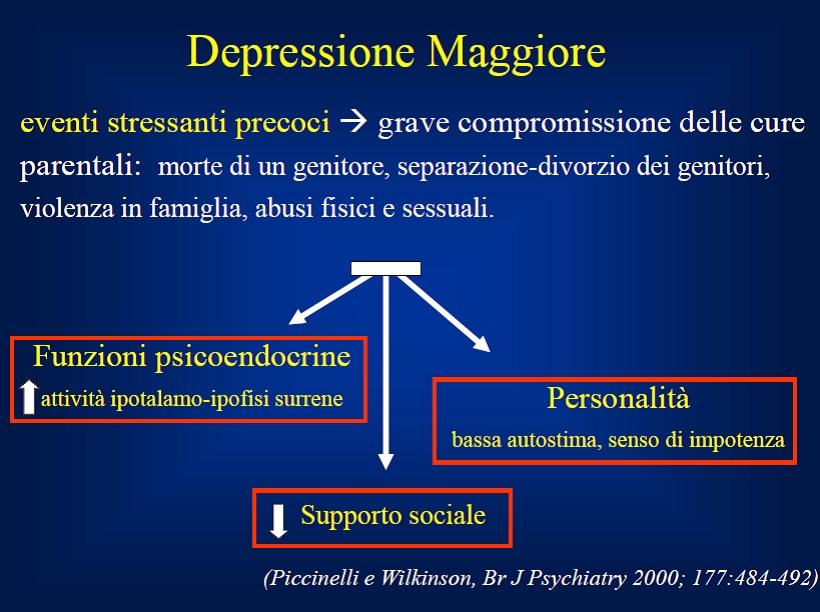
\includegraphics[width=0.9\textwidth]{02/image6.jpeg}
\end{figure}

\textbf{Consistono in tutto ciò che mette gravemente in crisi le cure
parentali}

\begin{itemize}
\item
  Malattie di un genitore
\item
  Morte di un genitore
\item
  Violenze in famiglia
\item
  Abusi fisici e sessuali
\end{itemize}

Non ci riferiamo ad eventi minori come il sospetto che mia mamma non mi
abbia voluto bene, abbia preferito mia sorella mio fratello o mi volesse
bionda; non è questo.

\emph{Considerazione sulle adozioni: è frequente riscontrare numerosi
eventi traumatici nella vita dei primi anni dei ragazzi adottivi; quello
che hanno vissuto potrebbe agire su un terreno geneticamente predisposto
ed ecco che i fattori di rischio che portano alla manifestazione della
malattia si accumulano. Per questo sarebbe opportuno fornire precise
informazioni circa i fattori di rischio alle famiglie che intendono
intraprendere un percorso di adozione, in maniera da poter effettuare
una scelta in maniera consapevole}. \emph{Il nostro cervello assorbe
anche quello che viene dall'ambiente. L'adozione non è una passeggiata,
l'ambiente famigliare non riesce ad annullare tutto ciò che hanno
vissuto nei primi mesi di vita e com'è il loro funzionamento cerebrale,
anche in relazione alla loro vulnerabilità ereditata dai genitori.}

\subparagraph{PERSONALITA'}

Per la depressione vale molto come fattore di rischio l'incapacità di
gestire le situazioni sociali.

Si può spiegare con una metafora: il mio modo di essere con gli altri è
come se fosse un auto, con un acceleratore che la fa muovere ed un freno
che ne riduce la velocità impedendole di andare a sbattere; se io ho un
sistema frenante molto più sviluppato del sistema di accelerazione
faccio molta fatica a muovermi. Il sistema frenate rappresenta il
timore, per esempio, di sbagliare, il timore di che cosa diranno gli
altri, il timore di rimetterci, essere danneggiato dalle scelte che
posso fare: allora sono molto cauto, circospetto, vado molto piano.
All'eccesso questo comportamento determina un disastro in termini di
situazioni sociali: è facile che abbia bisogno di qualcuno che faccia
andare l'acceleratore, di dipendere dagli altri. Questo determina una
forte compromissione delle abilità sociali, difficoltà a muoversi con
gli altri, inserito spesso in un quadro di regole assolute, rigide alle
quali il mondo deve aderire, scarsa flessibilità ed adattabilità agli
eventi esterni.

\begin{figure}[!ht]
\centering
	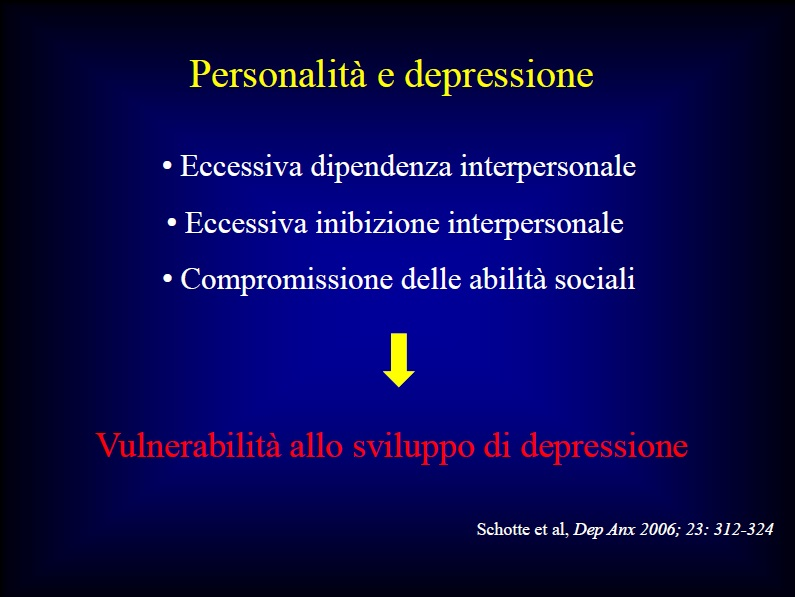
\includegraphics[width=0.9\textwidth]{02/image7.jpeg}
\end{figure}


\subparagraph{DISTURBI DI ANSIA}
Esiste una relazione tra disturbi depressivi e ansiosi

\begin{figure}[!ht]
\centering
	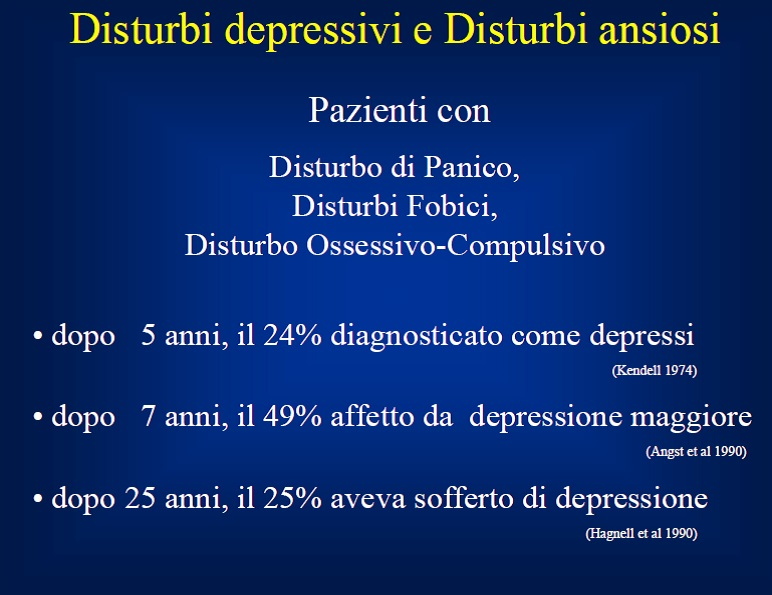
\includegraphics[width=0.9\textwidth]{02/image8.jpeg}
\end{figure}

I disturbi d'ansia possono rimanere tali ma più spesso cambiano, dopo 5
anni un quarto viene diagnosticato come depresso, dopo 7 anni
addirittura la metà. Il che vuol dire che, se io ho un disturbo d'ansia,
è facile che dopo alcuni anni sviluppi un episodio depressivo, anche
perché nella stessa famiglia disturbi ansiosi e depressivi vanno un po'
a braccetto: la famigliarità per uno mi espone ad un rischio anche nei
confronti dell'altro.

Se tolgo l'effetto dell'ansia, la differenza tra sesso maschile e
femminile si riduce del 50\% sulla frequenza di depressione: significa
che il fatto di aver sofferto d'ansia (ancora maggiore incidenza
femminile) è un fattore importante per aumentare nelle donne il rischio
di ammalarsi di depressione maggiore.

\subparagraph{DISTURBI SOMATICI}

Qui in realtà, se andiamo ad analizzare il profilo depressivo associato
a malattie somatiche, notiamo quadri abbastanza diversi dalla
depressione vera e propria, melanconica, presa in considerazione finora.

Interessante è quello che succede quando io ho una forma anche molto
lieve di depressione, addirittura sintomi che non arrivano alla soglia
della diagnosi vera e propria: l'impatto sull'evoluzione della malattia
è nefasto. Consideriamo uno studio su pazienti che hanno malattia
coronarica: tra questi quelli che hanno manifestato anche solo
\textbf{sintomi} depressivi in seguito alla manifestazione coronarica
sono soggetti ad una mortalità praticamente doppia rispetto agli altri.
Monitorando 100 pazienti in unità coronarica che hanno avuto un infarto,
alcuni di questi entro pochi mesi in genere manifestano sintomi
depressivi. A distanza di un anno si evidenzia che questi ultimi hanno
una probabilità doppia di essere deceduti rispetto agli altri; se alcuni
hanno manifestato una maggiore intensità di depressione (soglia
diagnostica) della durata di 3-6 mesi vado leggermente sopra al doppio,
da 6 mesi mi avvicino al triplo come probabilità di decesso. Peggioro
decisamente il decorso ed esito del disturbo coronarico, come anche di
tutte le patologie cerebrovascolari. Si sono evidenziati alcuni
meccanismi eziopatogenetici: non è tanto o solo perché il paziente non
prenda la terapia e non mantenga gli stili di vita corretti; la
depressione modifica l'aggregabilità delle piastrine, modifica l'heart
rate variability, l'attività elettrica cardiaca, l'attività delle
interleuchine e la cascata pro infiammatoria, i livelli di cortisolo e
noradrenalina. Quindi interverrebbe pesantemente nella patogenesi dell'
infarto e delle malattie cardiache.

\subparagraph{FATTORI SOCIO-CULTURALI}

\begin{figure}[!ht]
\centering
	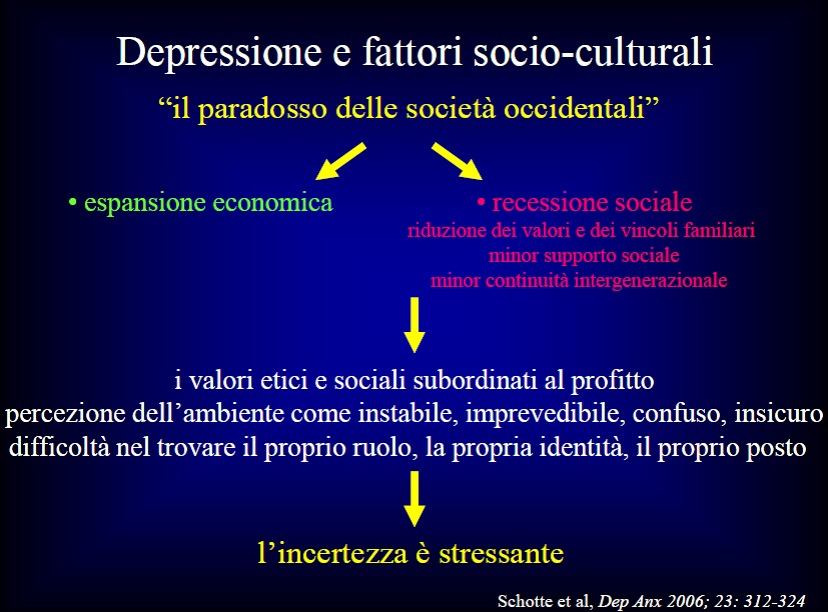
\includegraphics[width=0.9\textwidth]{02/image9.jpeg}
\end{figure}

Secondo alcuni la depressione sarebbe più frequente negli ultimi anni
rispetto a 100-50 anni fa. In parte è vero e l'incremento riguarda in
particolare le forme minori, più lievi. Uno psicologo ha preso in
considerazione l'odierna società, evidenziando come (specie in quella
occidentale) si abbiano è vero più possibilità economiche, ma anche
molta meno sicurezza sociale: lavoro, cambiamenti di ruolo, rete
sociale. Basti pensare a come il modello di famiglia odierno sia
diverso, per esempio, dalla famiglia patriarcale di una volta del mondo
contadino, dove c'erano 17-18 componenti e in cui, se uno non stava
bene, subentravano gli altri. Chiaramente questo modello paga un effetto
collaterale, ovvero il capofamiglia che decide per tutti, però li vi era
un supporto. Oggi la famiglia media italiana si compone di meno di 2
elementi: se uno si ammala ci si ritrova da soli. Se ci si ammala
bisogna riprendersi alla svelta, perché non c'è nessuno che possa
prendere il nostro posto e in queste condizioni diventa difficile
recuperare completamente. Bisogna considerare che anche queste forme
lievi hanno un certo impatto sul mio funzionamento e che non durano
pochissimo: parliamo di 3-4 settimane, a volte anche di più. Si ha la
possibilità di recupero? L'aumento, se è vero, c'è per le forme più
lievi ma le forme più gravi rimangono piuttosto stabili.

\subparagraph{Eventi stressanti}

Stiamo parlando del momento in cui passo dalla vulnerabilità alla
malattia.

Eventi di \textbf{perdita,} che può essere una perdita \emph{reale}:
morte di una persona a me cara o \emph{simbolica}, perdita del lavoro,
mancato raggiungimento di un obiettivo che il soggetto ritiene
importante, \textbf{elevati conflitti}. Sono tutti molto frequenti prima
di un episodio depressivo e rappresentano, molto probabilmente, il
momento in cui l'anfora tende a tracimare.

È sorto il problema di stabilire se l'evento sia \emph{reattivo}; è
possibile che vi siano episodi che intervengono nella vita di un
soggetto come fulmini a ciel sereno, però spesso c'è qualcosa che ci
induce quel meccanismo. Più che parlare di depressione reattiva, una
definizione un po' passata, interessa la sintomatologia perché quanto a
relazione tra evento di vita e quadro depressivo è molto più frequente
che ci sia un evento di vita, ma questo non vuol dire che quel quadro
sia comunque reattivo a quell'evento. In genere in passato \emph{la
depressione reattiva}, che si trova ancora nella classificazione, aveva
un particolare pattern sintomatologico: il soggetto era si triste ed
ansioso ma tutta la sua vita, quindi il suo umore, quello che pensava,
andava comunque a finire su quell'evento. Un esempio: mi lascio con il
fidanzato, quindi non sono allegro, faccio fatica a dormire. Se provo a
vedere tutto quello che penso e che mi impedisce di addormentarmi, noto
che può essere l'idea che forse ho sbagliato, forse sarebbe stato meglio
se avessi fatto questo, e non se avessi fatto quest'altro, ecc (la
cosiddetta \emph{polarizzazione dell'evento}).

Se considero invece un episodio depressivo come quelli presentati nelle
scorse lezioni (come l'avvocato per intenderci), posso aver avuto un
evento come il calo dei clienti, ma dall'esser calati i clienti a dire
che tutto corre solo ed unicamente su quel filone ce ne passa: non è
tutto legato a quell'evento.

È molto più frequente che io abbia un \emph{trigger} che innesca
l'episodio, mentre è molto meno frequente che quel quadro depressivo sia
strettamente connesso come sintomatologia, come manifestazione a
quell'evento: è possibile, ma raro.

Per \textbf{depressione reattiva} intendiamo quando un quadro
sintomatologico ha un'espressione in cui tutto quello che vive il
paziente è strettamente connesso, polarizzato su quell'evento.

Gli eventi di vita che abbiamo preso in considerazione sono invece
inneschi per trigger.

Una considerazione importante è sorta studiando il disturbo bipolare, in
cui si è visto che è molto più facile che gli episodi di malattia
iniziali siano in qualche modo scatenati da degli eventi. Man mano che
io avanzo si perde questa successione tra stimolo ed episodio; viene
meno l'effetto trigger di un evento e quindi è più facile che gli
episodi partano quando hanno voglia loro, in modo quasi spontaneo.

In un esperimento si sono provocate delle crisi epilettiche ad un
animale da esperimento con la stimolazione elettrica: dopo un certo
numero di scosse l'animale fa le crisi epilettiche da solo. Il modello
applicato al disturbo bipolare è che si ha inizialmente uno stimolo e
successivamente l'episodio; dopo un certo numero di stimoli il mio
cervello mette in atto delle crisi indipendentemente dallo stimolo
esterno.

\textbf{Chiaramente i fattori di rischio devono modificare il
funzionamento cerebrale: la risonanza magnetica funzionale di uno stesso
paziente fatta quando lui sta bene (in eutimia) e fatta quando è
depresso, non è la stessa}.

Consideriamo uno studio fatto dal professor Parmigiani con la
collaborazione dell'unità di psichiatria sui topi, i quali hanno un
sistema gerarchico in cui il ``topo secondo'' non attacca il ``primo''.
Ad un certo punto è stato iniettato del viagra al topo secondo, che
attacca e vince il primo. L'ex topo primo si mette in disparte con la
coda tra le gambe. Gli hanno tagliato la testa e sono andati a vedere
cosa succedeva nel cervello: il dosaggio del BDNF (fattore di crescita
neuronale) risulta abbassato, le aree ippocampali si sono ridotte. Il
sistema cerebrale del povero topolino si è modificato e questo soltanto
in forza di uno stimolo sociale, ambientale: ha cambiato solamente di
rango. Il nostro sistema cerebrale non è autonomo, non è sigillato
dall'ambiente, altrimenti non si capirebbero tutti questi fattori di
rischio che modificano il funzionamento del nostro cervello.

Per quanto riguarda i meccanismi che sono alla base dell'insorgenza
della manifestazione depressiva, vari studi hanno ormai messo in luce
con chiarezza che si tratta di un \textbf{\emph{processo
eziopatogenetico complesso}}, in cui rientrano sicuramente delle
componenti di \emph{ereditarietà}, che predispongono allo sviluppo del
disturbo dell'umore, ma su cui vanno poi ad agire anche altri fattori,
quali il \emph{sesso}, gli eventuali \emph{eventi traumatici precoci},
lo \emph{stress}, i \emph{fattori socio-economici e culturali}, le
\emph{malattie somatiche} e la \emph{personalità} del paziente stesso.

\subsubsection{Altre forme di depressione}

Accanto alla Depressione Maggiore, che rappresenta comunque il quadro
clinico più comune e rilevante dal punto di vista epidemiologico, in
base ai criteri del DSM sono state stabilite anche alcune varianti
dell'episodio depressivo, rispettivamente la \emph{depressione con
manifestazioni melanconiche}, la \emph{depressione con manifestazioni
psicotiche}, la \emph{depressione con manifestazioni catatoniche}, la
\emph{depressione con manifestazioni atipiche}, la \emph{depressione
breve ricorrente} e la \emph{depressione minore}.

\paragraph{Depressione con Manifestazioni Melanconiche}
  Corrisponde essenzialmente con la vecchia depressione endogena della
  nosografia classica, e si caratterizza per la \emph{peculiarità e la
  gravità dei sintomi}, nonché per la \emph{buona risposta ai
  trattamenti somatici} (TEC e antidepressivi), per l'\emph{assenza di
  eventi scatenanti} e per il \emph{buon funzionamento della personalità
  in epoca premorbosa e nelle fasi di remissione}.

  Secondo i criteri del DSM-IV, si può parlare di depressione
  melanconica quando vi è almeno uno dei seguenti sintomi principali:

\begin{itemize}
\item
  \emph{Perdita di piacere per tutte o quasi tutte le attività
  quotidiane;}
\item
  \emph{Perdita di reattività agli stimoli abitualmente piacevoli.}
\end{itemize}

In più, devono anche essere presenti almeno \emph{3 dei seguenti
sintomi}:

\begin{itemize}
\item
  \emph{Una specifica qualità dell'umore depresso, che risulta quindi
  nettamente distinto dal tipo di sentimento provato ad esempio dopo la
  perdita di una persona cara;}
\item
  \emph{Depressione regolarmente peggiore al mattino;}
\item
  \emph{Risveglio precoce al mattino} (almeno 2 ore prima del solito);
\item
  \emph{Marcato rallentamento motorio o agitazione;}
\item
  \emph{Anoressia o perdita di peso;}
\item
  \emph{Sentimenti di colpa inappropriati o eccessivi.}
\end{itemize}

\paragraph{Depressione con Manifestazioni Catatoniche}
In questo
  sottotipo sono in primo piano i \emph{sintomi psico-motori}, come il
  grave rallentamento che può arrivare sino alla catalessia, alla
  flessibilità cerea ed allo stupor. Non sono rari nemmeno i movimenti
  stereotipati, i manierismi e l'assunzione di posture inadatte o
  bizzarre, talvolta anche con ecoprassia o ecolalia.

  In base ai criteri del DSM, il quadro clinico è dominato da almeno 2
  dei seguenti sintomi:
  
\begin{itemize}
\item
  \emph{Immobilità}, come evidenziato dalla \emph{catalessia}, dalla
  \emph{flessibilità cerea} o dallo \emph{stupor};
\item
  \emph{Eccessiva attività motoria}, afinalistica e non correlata agli
  stimoli esterni;
\item
  \emph{Negativismo estremo o mutacismo;}
\item
  \emph{Peculiarità dei movimenti volontari}, come evidenziato dal
  mettersi in posa, dai manierismi e dai movimenti stereotipati;
\item
  \emph{Ecolalia o ecoprassia.}
\end{itemize}

In ogni caso, la depressione con manifestazioni catatoniche è una
\emph{forma particolarmente grave}, per cui è necessario il ricovero in
ambiente specialistico e che può talvolta richiede l'impiego della
terapia elettroconvulsivante.

\paragraph{Depressione con Manifestazioni Psicotiche}
È una forma
  che costituisce circa il 10\% di tutte le forme depressive, la cui
  sintomatologia \emph{si associa a deliri e/o allucinazioni}, il cui
  contenuto può essere \textbf{congruo} o \textbf{incongruo} all'umore:
  nel primo caso abbiamo i tipici deliri di colpa, rovina e ipocondria,
  mentre nel secondo caso predominano i deliri di veneficio,
  persecuzione ed influenzamento. La depressione psicotica si manifesta
  in soggetti con un forte carico genetico, e comporta una lunga durata
  degli episodi ed un alto rischio di suicidio, per cui richiede in
  genere l'ospedalizzazione e tende a ripresentarsi sempre con le stesse
  caratteristiche anche agli episodi successivi, in genere richiedendo
  anche la somministrazioni di antipsicotici o il ricorso alla TEC.

\paragraph{Depressione con Manifestazioni Atipiche}
Si tratta di
  una forma depressiva il cui quadro clinico può essere considerato come
  l'opposto di quello presente nella depressione con melanconia, in
  quanto \emph{l'umore appare reattivo e tende a mutare in relazione
  agli stimoli esterni,} ma c'è un'eccessiva sensibilità al rifiuto che
  influenza negativamente i rapporti sociali ed il lavoro, spesso
  causando un stile di vita burrascoso, colpendo con frequenza
  leggermente superiore i soggetti di sesso femminile. In base ai
  criteri del DSM-IV, infatti deve essere presente una chiara reattività
  dell'umore, in associazione con 2 o più delle seguenti
  caratteristiche:

\begin{itemize}
\item
  \emph{Significativo incremento ponderale o aumento dell'appetito;}
\item
  \emph{Ipersonnia;}
\item
  \emph{``Paralisi Pleumbea'',} cioè sensazione di pesantezza o di avere
  le braccia e le gambe di piombo;
\item
  \emph{Quadro duraturo di ipersensibilità al rifiuto interpersonale,
  non limitato agli episodi di alterazione del tono dell'umore, che
  causa una compromissione sociale o lavorativa significativa.}
\end{itemize}

Inoltre, non devono essere soddisfatti i criteri per la depressione con
manifestazioni melanconiche o catatoniche.

La depressione atipica, purtroppo, è una forma difficile da
\emph{trattare}, e necessita sia di un trattamento farmacologico con
SSRI o IMAO sia di un accurato approccio psico-terapeutico.

\paragraph{Depressione Breve Ricorrente}
In questa forma
  depressiva sono soddisfatti gli \emph{stessi criteri che nella
  depressione maggiore}, con la sola differenza che i sintomi devono
  essere contemporaneamente presenti per \emph{meno di 2 settimane} e
  devono comunque rappresentare un cambiamento rispetto al precedente
  livello di funzionamento.

\paragraph{Depressione Minore}
Anche in questo caso si tratta di
  una variante ``depotenziata'' della depressione maggiore, da cui
  differisce per il fatto che vi sono \emph{da 2 a 4 sintomi} (di cui
  almeno uno è l'umore depresso o la perdita di interesse e piacere) che
  coesistono contemporaneamente per almeno 2 settimane.


Oltre alla depressione maggiore e alle varianti ad essa correlate,
esistono poi anche altri disturbi dell'umore in senso prevalentemente o
unicamente depressivo, rappresentati dal \textbf{disturbo dell'umore ad
andamento stagionale} ed i \textbf{disturbi depressivi del puerperio}.


\paragraph{Disturbo dell'Umore ad Andamento Stagionale}

  È una forma di disturbo dell'umore relativamente comune che, in base
  ai criteri del DSM, si caratterizza la \emph{presenza di una relazione
  temporale regolare tra l'esordio degli episodi depressivi maggiori o
  con le fasi depressive del disturbo bipolare}, in particolare per
  quanto riguarda l'\textbf{\emph{andamento stagionale}} (ad esempio si
  ha una regolare comparsa dell'episodio depressivo in autunno-inverno,
  ed una sua attenuazione con la bella stagione), e anche le remissioni
  della patologia avvengono in base alle variazioni della stagione o in
  un determinato periodo dell'anno. Inoltre, \emph{negli ultimi 2 anni
  si devono essere presentati almeno due episodi depressivi maggiori che
  rispettano la relazione temporale sopra illustrata}, \emph{senza che
  via sia alcun episodio depressivo maggiore non stagionale} nello
  stesso periodo e, qualora il paziente avesse avuto nel corso della
  vita anche episodi depressivi non stagionali, il numero di questi deve
  essere significativamente inferiore rispetto a quello degli episodi
  stagionali.


\paragraph{Disturbo Depressivi del Puerperio}

  Il parto ed il post-partum rappresentano un periodo estremamente
  stressante sia per il neonato che per la madre, la quale può
  sviluppare delle forme di disturbo dell'umore di gravità variabile,
  che fortunatamente si risolvono però nel giro di alcuni giorni o
  settimane. In linea di massima, non è così inusuale riscontrare
  recidive di disturbo bipolare, di depressione maggiore o anche di
  psicosi brevi entro 4 settimane dal parto, ma esistono anche delle
  forme depressive più specifiche che interessano questo periodo della
  vita della donna, che sono i cosiddetti ``Maternity Blues'', la
  depressione maggiore ad esordio nel post-partum e la psicosi
  puerperale.

\begin{itemize}
\item
  \textbf{\emph{Maternity Blues}}: Sono \emph{forme depressive
  relativamente comuni}, che arrivano ad interessare sino al 50-85\%
  delle donne , esordendo \emph{entro pochi giorni dal parto} (in genere
  entro 48 ore), e si manifestano con tristezza, facilità al pianto,
  sentimenti di insicurezza e di incapacità, ansia, irritabilità,
  difficoltà di concentrazione e nella memoria, disturbi dell'appetito,
  della memoria, cefalea ed astenia. In genere vanno in remissione entro
  2 settimane, in caso si protraessero più a lungo è bene sospettare la
  loro evoluzione a depressione post-partum.
\item
  \textbf{\emph{Depressione Post-Partum}}: È una \emph{forma depressiva
  che esordisce entro 3 mesi dal parto, in genere entro il primo mese},
  ed ha una prevalenza nella popolazione delle puerpere del 10-22\%; dal
  punto di vista sintomatologico è del tutto sovrapponibile alla
  depressione maggiore, e in genere va incontro a \emph{remissione
  spontanea entro 6-12 mesi}, sebbene vada trattata per i suoi possibili
  effetti sullo sviluppo psichico del bambino, che potrebbe sviluppare
  un atteggiamento insicuro ed ambivalente, con compromissione del tono
  emozionale e dello sviluppo cognitivo e relazionale, nonché
  manifestazioni psicopatologiche tardive.
\item
  \textbf{\emph{Psicosi Post-Partum}}: Interessa fortunatamente solo lo
  0,1-0,3\% di tutte le puerpere, esordendo \emph{entro al prima
  settimana dal parto} (in genere entro le prime 72 ore).
  Sintomatologicamente si caratterizza per la presenza di intense e
  rapide oscillazioni dello stato di coscienza, con allucinazioni visive
  o uditive a contenuto triste o terrifico, temi deliranti di tipo
  persecutorio o depressivo, in genere incentrati sulla relazione
  madre-bambino, tali da determinare ansia ed agitazione. È una forma
  nettamente più preoccupante delle due precedenti, poiché correlata con
  un \emph{rischio non indifferente di suicidio ed infanticidio}; ciò
  nonostante la prognosi è relativamente buona, con \emph{remissione
  entro 6-12 mesi} dall'esordio nell'80\% dei casi, sebbene tenda a
  ripresentarsi nei successivi periodi post-partum, e nel 70\% dei casi
  possa poi preludere a manifestazioni depressive o bipolari con
  caratteri psicotici.
\end{itemize}

\subsubsection{Sottotipi di depressione (secondo il Maggini)}

Secondo la psicopatologia classica, all'interno delle sindromi
distimiche, e più nello specifico nell'ambito della depressione, è
possibile identificare alcune forme specifiche sulla base
dell'eziopatogenesi, delle manifestazioni cliniche e del decorso ad esse
associate; in questa suddivisione rientrano pertanto la
\emph{depressione endogena}, la \emph{depressione psicogena}, la
\emph{depressione endoreattiva}, la \emph{depressione mascherata} e
quella \emph{somatogena}, a cui viene qui associata anche la descrizione
della \emph{depressione infantile} e quella \emph{dell'età involutiva}.

\paragraph{Depressione Endogena}

La \textbf{depressione endogena}, così come descritta nei testi di
psichiatria e psicopatologia classica, è una forma depressiva in cui
\emph{non è possibile identificare un precedente avvenimento di vita che
possa essere considerato obiettivamente significativo}, per cui non
esiste alcun rapporto di comprensibilità fra lo stato depressivo e la
situazione pre-depressiva. Questa condizione depressiva, peraltro, si
caratterizza in genere per una \emph{notevole tristezza vitale}, che
irrompe in maniera psicologicamente e biograficamente priva di senso,
all'improvviso, e in genere ha un \emph{decorso fasico}, a frequenza più
o meno elevata, con caratteristiche periodiche, accompagnandosi ad
alcuni tipici \emph{disturbi somatici}, come insonnia, dimagrimento,
disturbi del ciclo mestruale e diversi altri. La depressione endogena,
secondo la psicopatologia classica, è inoltre considerata come una
\textbf{somatosi}, cioè una \emph{malattia riconducibile ad una base
somatica ancora in gran parte sconosciuta}, che negli ultimi anni si è
tuttavia visto risiedere probabilmente in una certa predisposizione
genetica a base ereditaria, su cui possono poi andare ad agire fattori
ambientali scatenanti.

Dal punto di vista clinico, la depressione endogena si sovrappone per
buona parte alla depressione maggiore ricorrente, caratterizzandosi per
\emph{sentimenti di tristezza immotivata}, \emph{inaridimento e
svuotamento affettivo}, \emph{arresto del tempo interiore} e alterazioni
anche molto marcate del vissuto corporeo, e non va dimenticato il
terribile ``\textbf{sentimento di mancanza di sentimenti}'', che risulta
notevolmente angosciante per questi soggetti, così come lo è il loro
\textbf{vissuto del tempo interiore}, da cui possono scaturire intenti
suicidari o autolesionistici. Sul piano comportamentale si coglie
un'\emph{inerzia psicomotoria}, una forte tendenza all'isolamento con
riduzione dei gesti, della mimica, del linguaggio verbale e del
pensiero.

N.B.: Accanto alla depressione endogena, la psicopatologia classica
classifica nelle forme endogene anche il \emph{disturbo bipolare},
poiché anche questa condizione non riconosce alcuna causa esogena alla
sua base, per cui nelle distimie endogene devono essere considerate sia
le forme unipolari che quelle bipolari.

\paragraph{Depressione Psicogena}

Le \textbf{depressioni psicogene} sono un gruppo eterogeneo di disturbi
dell'umore che sono \emph{riconducibili ad un evento di particolare
significato esistenziale} (\textbf{depressione reattiva}) o
all'\emph{elaborazione depressiva di conflitti inconsci riattivati da
una situazione attuale} (\textbf{depressione nevrotica}).

Le depressioni psicogene si contrappongono pertanto classicamente a
quelle endogene per aspetti eziopatogenetici, sintomatologici ed
evolutivi: se nelle forme endogene si ha un fondamento biologico sotto
forma di predisposizione ed una marcata mancanza di motivazioni, nelle
forme psicogene si riconoscono \emph{diversi meccanismo psicogenetici} e
la \emph{presenza di eventi o situazioni conflittuali}, inoltre, mentre
nelle forme endogene il vissuto depressivo si manifesta con inibizione
psicomotoria e tristezza vitale, nella depressione psicogena si
manifesta invece con \emph{irrequietudine ansiosa} ed \emph{alterazioni
dei sentimenti psichico-spirituali}. Infine, se le forme endogene
presentano un andamento fasico e periodico, quelle psicogene mostrano
spesso un \emph{decorso protratto o cronico}.

Il \textbf{decorso} della depressione psicogena, inoltre, \emph{è in
stretta relazione con gli avvenimenti di vita che l'hanno scatenata},
per cui non è generalmente prevedibile in base alla sola anamnesi, e le
ricadute sono fortunatamente meno frequenti che nelle depressioni
endogene. Elemento fondamentale della depressione psicogena è il fatto
che il paziente è \emph{consapevole della propria malattia}, per cui si
manifesta accessibile al contatto interumano. Clinicamente, il quadro è
molto \emph{polimorfo e mutevole}: in genere non compaiono temi di
autoaccusa o di svalutazione, e le pulsioni aggressive, se presenti,
sono rivolte verso gli altri, mentre i possibili propositi autolesivi,
sebbene rari, si manifestano in maniera teatrale, con intenti
protestatari ed aggressivi nei confronti dell'ambiente. Frequenti sono
anche le lamentele somatiche, con disturbi gastro-intestinali, cardiaci
e respiratori, e comuni sono anche i fenomeni neuro-vegetativi ed i
disturbi del sonno.

\paragraph{Depressione Endoreattiva}

Nota anche come \textbf{distimia endoreattiva di Weitbrecht}, questa
forme di depressione può essere considerata come l'anello di
congiunzione tra la depressine endogena e la depressione psicogena
reattiva, infatti in questa forma il disturbo dell'umore \emph{si
sviluppa inizialmente come una reazione ad un evento di vita, ma
prosegue poi evolvendo ad una forma che può essere a tutti gli effetti
considerata endotimica}, tanto che nelle fasi più avanzate non la si
riesce più a distinguere dalla depressione endogena propriamente detta.
I soggetti che sviluppano questa depressione endoreattiva sono
tipicamente soggetti con una \emph{personalità pre-morbosa}
caratterizzata da tratti di tipo astenico, delicato-esauribile, o
irritabile-sensitivo, in ogni caso poco socievole, per cui sono soggetti
facili alle depressioni immotivate ed alle reazioni disforiche.

L'evento scatenante può avere caratteristiche estremamente variabili, ad
esempio può consistere nello sradicamento dall'ambiente consuetudinario,
come nei trasferimenti in posti lontani, oppure le persecuzioni
politiche o razziali, la frattura del nucleo familiare con perdita di
persone care, ma non bisogna dimenticare anche eventi di natura
somatica, come le gravidanze complicate e gli aborti ripetuti, le
convalescenze prolungate per malattie infettive o malattie croniche
debilitanti. Lo stato d'animo del paziente viene tipicamente definito
come quello di una \textbf{tristezza astioso-lamentosa}, con un paziente
che viene definito spesso come ``\emph{disforico ed adirato}'', e che
tende ad abbandonarsi ad un'ipocondria lamentosa, la quale tuttavia non
raggiunge mai i livelli deliranti estremi dei deliri nichilistici o
della sindrome di Cotard. Il decorso della depressione endoreattiva,
infine, è protratto e la fine dell'episodio è mal definibile, infatti
non si osserva una risoluzione rapida come nella depressione endogena,
né un viraggio verso lo stato maniacale, e la risoluzione avviene per
lisi graduale, con ritorno allo stato pre-morboso.

\paragraph{Depressione Somatogena}

Detta anche \textbf{depressione organica}, è un quadro depressivo in cui
è possibile identificare un \emph{rapporto causale con una patologia
somatica} che può o interessare primariamente il SNC o interessare
organi ed apparati al di fuori del cervello, ma che riescono a
provocare, per vie secondarie, alterazioni a livello di questo
distretto.

Tra le patologie che coinvolgono primariamente il SNC si possono
riconoscere diverse condizioni, come \emph{fenomeni atrofici},
\emph{tumori}, \emph{crisi epilettiche} e \emph{meningo-encefaliti}, ma
in primo piano sono le affezioni che coinvolgono le strutture
sottocorticali e, nello specifico, il \textbf{diencefalo}, come
dimostrato dal fatto che fra i tumori cerebrali, quelli che più
comunemente danno manifestazioni depressive sono i tumori che si
sviluppano in corrispondenza del tronco encefalico, seguiti poi dalle
neoplasie dei lobi frontale e temporale. Numerose condizioni morbose
extracerebrali sono poi ritenute responsabili della comparsa di uno
stato depressivo, e tra queste devono essere ricordate varie
\emph{patologie cardiache}, \emph{renali}, \emph{ematiche} e forme
\emph{neoplastiche}, ma particolare rilievo hanno le
\textbf{\emph{endocrinopatie}}, come dimostrato dal fatto che alcune
patologie, come la sindrome di Cushing o il morbo di Addison sono
correlati con manifestazioni disti miche, mentre le variazioni dei
livelli di ormoni tiroidei possono anch'essi dare disturbi dell'umore
(più nello specifico, l'ipotiroidismo dà manifestazioni depressive,
mentre l'ipertiroidismo manifestazioni ipomaniacali o francamente
maniacali). Particolare attenzione va poi posta ai
\textbf{\emph{trattamenti farmacologici}}, che possono dare
manifestazioni di depressione somatogena, in particolare alcuni agenti
ipotensivi oggi poco usati, come la reserpina e l'$\alpha$ -metil-DOPA, ma anche
i cortisonici, i contraccettivi orali ed i neurolettici (soprattutto la
flufenazina in somministrazione depot).

Il quadro clinico della depressione somatogena si caratterizza per
l'essere \emph{relativamente povero di sintomi affettivi}: al posto
della tristezza vitale si può infatti cogliere uno \emph{stato
astenico-apatico} o \emph{iperestesico-disforico}, con povertà di
contenuti depressivi profondi e con malumore insistente, monotono e
associato a lamentosità. Tipicamente \emph{manca anche la profondità del
sentimento di colpa}, così come la sconvolgente disperazione
esistenziale, che sono invece tipici della depressione endogena.

Per la diagnosi della depressione somatogena è necessario che siano
rispettati i seguenti criteri:

\begin{itemize}
\item
  \textbf{Dev'essere presente una patologia organica cerebrale o
  extracerebrale};
\item
  \textbf{Dev'esserci uno stretto rapporto cronologico tra la malattia
  somatica e lo stato depressivo};
\item
  \textbf{Devono essere presenti sintomi psico-organici, come disturbi
  dello stato di coscienza o disorientamento spazio-temporale};
\item
  \textbf{Si devono riscontrare delle peculiarità fenomenologiche dello
  stato depressivo, come quadri di tipo astenico-ipobulico o
  iperestesico-disforico};
\item
  \textbf{Si deve riscontrare una risposta al trattamento specifico,
  come ad esempio ormonip o agenti anti-infettivi}.
\end{itemize}

In ogni caso, queste forme depressive sono \emph{sensibili alle terapia
specifiche}, capaci di incidere sulla malattia organica alla base,
sebbene non sia infrequente che lo stato depressivo possa rispondere al
trattamento farmacologico antidepressivo. L'evoluzione e la prognosi
della depressione somatogena sono comunque grandemente determinate dalla
patologia organica primitiva.

\paragraph{Depressione Mascherata}

Nota anche col nome di ``\textbf{equivalente depressivo}'', è un
\emph{particolare disturbo dell'umore che si mantiene coperta},
``\emph{mascherata}'', \emph{da sintomi somato-vegetativi}, nonché
alterazioni comportamentali o altre eterogenee sindromi
psicopatologiche. Dal punto di vista psicogenetico, le depressioni
mascherate sono da considerarsi come delle particolari forme di
depressione su base endogena, in cui prevale tuttavia una
\emph{sintomatologia somatica molto marcata}, la quale finisce per
celare il vissuto depressivo, e a cui si possono peraltro associare
anche altre manifestazioni psichiche e comportamentali.

La depressione mascherata è una \textbf{condizione tipica
dell'infanzia}, in cui l'angoscia depressiva si può manifestare solo
sotto forma di equivalente depressivo, infatti si è visto che solo
dall'adolescenza (o almeno a partire dai 10 anni) si riscontrano vissuti
di tristezza, di solitudine, di colpa e quadri sindromici assimilabili
alla depressione classicamente intesa. Anche nell'\textbf{età
involutiva} si riscontra una maggior incidenza della depressione
mascherata, poiché negli anziani le comorbilità sono molto frequenti, e
spesso il soggetto tende a riferire i suoi disturbi distimici ai
problemi somatici. Tipiche sono quindi le \emph{manifestazioni di tipo
fobico-ossessivo}, \emph{neurastenico-cenestopatiche}, ma anche
\emph{algiche} o \emph{isteriche}, che si vanno a sommare alle
manifestazioni somatiche, che sono comunemente rappresentate da
\emph{disturbi gastro-intestinali}, \emph{disturbi genito-urinari},
\emph{cardiovascolari} e \emph{respiratori}.

La \textbf{diagnosi} di depressione mascherata si avvale del
\emph{rilievo di sintomi di tipo depressivo}, della \emph{valutazione} e
delle \emph{caratteristiche evolutive del quadro clinico}, nonché del
\emph{criterio ex-adjuvantibus}, poiché questa forma depressiva risponde
relativamente bene agli antidepressivi triciclici e tetraciclici, che
rappresentano i principali presidi terapeutici.

\paragraph{Depressione dell'Età Infantile}

Per molto tempo si è erroneamente ritenuto che i bambini godessero di
una qualche immunità per le malattie psichiche che colpiscono gli
adulti, tra cui anche la depressione. In realtà, a partire dal XVII
secolo, si è visto che i bambini possono sviluppare anch'essi delle
forme depressive, ed inizialmente si credeva che queste fossero la
conseguenza di un'alterazione dovuta a fattori socio-ambientali, ma oggi
questa ipotesi non è più sostenibile.

Per quanto riguarda l'epidemiologia della depressione infantile, la sua
incidenza reale tende ad essere mal definita, poiché queste forme
depressive \emph{non rispettano generalmente i criteri usati per porre
diagnosi di depressione negli adulti}, infatti il bambino, soprattutto
se piccolo, non riesce a manifestare quadri psicopatologici
sovrapponibili a quelli dell'adulto, a causa dell'assenza o la riduzione
del versante soggettivo inerente al suo vissuto interiore, e non possono
nemmeno esprimere quello che provano in maniera verbale, motivo per cui
queste forme depressive sono esternate con \emph{agitazione} anche molto
marcata, con un \emph{modo preverbale} o con un \emph{linguaggio
mimico-gestuale-motorio}, nonché con le \emph{manifestazioni somatiche},
da cui si sviluppa appunto la \textbf{depressione mascherata}.

Gli aspetti dalla depressione infantile tendono a differire notevolmente
in base all'\emph{età} del paziente: nella \textbf{\emph{prima
infanzia}} si hanno tipicamente delle \emph{turbe dell'alimentazione o
del sonno}, \emph{ritardo dello sviluppo psicomotorio} e, nei casi più
gravi, \emph{decadimento delle condizioni somatiche generali}. Il più
precoce comportamento depressivo nell'infanzia è quello definito di
``\textbf{depressione anaclitica}'', che insorge nel \emph{primo}
\emph{anno di vita} in bambini separati dalla madre: in una prima fase i
bambini diventano \emph{piagnucolosi}, \emph{esigenti}, e cercano di
aggrapparsi ad ogni persona; la loro espressione del volto è di evidente
\emph{tristezza}, e vi è \emph{perdita di pero ed arresto dello sviluppo
corporeo}. Successivamente, i bambini rifiutano qualsiasi contatto
interumano e la mimica si irrigidisce, associandosi ad una continua
perdita di peso e ritardo motorio sino ad uno stato simil-letargico. Se
entro qualche mese il bambino viene affidato ad un accettabile sostituto
materno i disturbi scompaiono velocemente, altrimenti il processo
continua sino allo \emph{stato di marasma}.

Nella \textbf{\emph{seconda infanzia}}, invece, la depressione si
manifesta con \emph{insufficienza delle prestazioni intellettive},
\emph{tendenza all'isolamento}, \emph{crisi di pianto immotivate} e si
possono anche rilevare \emph{condotte aggressive}, esasperazione delle
fisiologiche manifestazioni fobiche e comportamenti regressivi, mentre
in età scolare predomina il cattivo adattamento scolastico con ritardo e
difficoltà d'apprendimento. Solo a partire dai 10 anni in poi la
depressione assume caratteri di maggiore completezza ed acquista aspetti
simili a quella dell'età adulta, con comparsa di tristezza vitale,
blocco delle iniziative e dell'ideazione e depersonalizzazione
affettiva.

Sempre tra le manifestazioni depressive dell'infanzia va poi inclusa
anche la cosiddetta ``\textbf{Sindrome di Charlie Brown}'', in cui il
soggetto giunge ad un'\emph{accettazione rassegnata di un'esistenza
candidata al fallimento ed alla solitudine}, come nel personaggio di
Schultz, con fatalistica acquiescenza ed accettazione della propria
incapacità a dominare la realtà.

L'approccio terapeutico è essenzialmente farmacologico, a base di
\emph{antidepressivi triciclici} (se possibile, anche se oggi si
preferiscono gli SSRI) ed \emph{ansiolitici}, anche se utile è anche la
psicoterapia.

\paragraph{Depressione nell'Età Involutiva}

La depressione è una patologia purtroppo molto comune nella popolazione
anziana, sia perché questi pazienti sono più esposti a comorbilità molto
rilevanti e ad andamento cronico e progressivo, sia perché col tempo è
normale che il substrato sociale del paziente vada diradandosi, mentre
aumentano gli eventi di vista spiacevoli. Più nello specifico, vari
autori hanno evidenziato come l'età involutiva possa agire in diversi
modi nel determinare l'insorgenza dei disturbi dell'umore: secondo
alcuni l'invecchiamento favorirebbe la \emph{rivelazione di una
disposizione timopatica pre-esistente}, e ciò spiega anche il ripetersi
degli episodi maniaco-depressivi anche in età tardiva e l'inizio non
raro della depressione melanconica in età avanzata, secondo altri invece
il meccanismo principale risiede nel fatto che la vecchiaia \emph{espone
ad un numero rilevante di eventi di vita spiacevoli}, come perdite e
lutti, così come a \emph{turbe della sfera emotiva}, nonché a
\emph{malattie organiche di diversa natura}. Inoltre, come evidenziato
da altri autori, con l'invecchiamento i disturbi timici già presenti o
che si sviluppano in questa fase \emph{tendono a cristallizzarsi e
cronicizzarsi in maniera marcata e rapida}, per cui risultano molto più
difficili da trattare.

\subsubsection{Disturbo bipolare}

Si tratta di una particolare patologia psichiatrica, caratterizzata da
\emph{alterazioni del tono dell'umore ora in senso depressivo} (più
comuni) \emph{ora in senso manicale} (disturbo bipolare di tipo I)
\emph{o ipomaniacale} (disturbo bipolare di tipo II), \emph{o anche
episodi misti}.

Si possono avere quindi due forme:

\begin{itemize}
\item
  \textbf{DISTURBO BIPOLARE 1} (fase depressiva + maniacale) rapporto
  tra un episodio maniacale e uno depressivo è 1:3.
\item
  \textbf{DISTURBO BIPOLARE 2} (fase depressiva + ipomaniacale) rapporto
  tra un episodio ipomaniacale e uno depressivo è 1:8-1:12.
\end{itemize}

\emph{Sono disturbi diversi:} Si tenga presente che ciascun soggetto ha
il suo andamento e la sua frequenza, comunque in entrambe le forme il pz
vivrà più a lungo in fase depressiva piuttosto che in fase maniacale o
ipomaniacale e questo avviene soprattutto nel tipo 2.

ll bipolare 2 assomiglia ad un disturbo depressivo maggiore con episodi
frequenti e qualche episodio maniacale, si può avere anche un solo
episodio maniacale o ipomaniacale ogni 37 episodi depressivi.

Nel disturbo bipolare devono poi essere ricondotti anche gli episodi di
\textbf{``\emph{falso disturbo unipolare}''}, in cui abbiamo un paziente
che è affetto da episodi depressivi ricorrenti che nel tempo però
tendono a sviluppare mania o ipomania, tanto che dal 10 al 28\% delle
depressioni maggiori ricorrenti sono false depressioni unipolari.
Elementi che fanno pensare di essere di fronte non tanto ad un disturbo
unipolare ma uno di tipo bipolare sono:

\begin{itemize}
\item
  la familiarità bipolare,
\item
  il temperamento ipertimico o ciclotimico,
\item
  l'esordio precoce,
\item
  l'andamento stagionale, specie per quanto riguarda l'inibizione
  psicomotoria e l'ipersonnia,
\item
  l'elevata frequenza degli episodi,
\item
  l'esordio e la risoluzione improvvisa degli stessi,
\item
  l'ipomania indotta dagli antidepressivi TCA
\item
  la risposta al litio.
\end{itemize}

In genere, i pazienti hanno 10 o più episodi nel corso della vita, e la
durata della remissione tende a ridursi dal secondo episodio in poi, per
cui si può dire che il rischio di ricaduta è maggiore all'aumentare del
numero di episodi precedenti e nel post-partum (rischio 8 volte
maggiore).

\emph{Rispetto alla depressione unipolare ricorrente}, il disturbo
bipolare ha:

Una \textbf{frequenza elevata} degli episodi (circa 10 nel corso della
vita).

Un'insorgenza più precoce:Il disturbo bipolare esordisce in tarda
adolescenza o al più nella prima giovinezza: tra i 20 e i 30 anni
(mentre la depressione ricorrente più facilmente compare dopo i 30
anni).

Nella fase depressiva la sintomatologia è assolutamente sovrapponibile
(con un prevalere dell'inibizione, del rallentamento psicomotorio, e con
un maggior rischio di suicidio).

Sesso: Il \textbf{disturbo bipolare di tipo I}, meno comune, ha la
stessa frequenza in entrambi i sessi, mentre nel \textbf{disturbo}
\textbf{bipolare di tipo II} vi è una maggior frequenza nel sesso
femminile.

Per fare una diagnosi di pz bipolare il primo episodio deve essere
maniacale o misto, se invece si manifesta un episodio depressivo è
difficile poter preventivare, anche se si hanno degli elementi che
possano far supporre che questo soggetto sia un bipolare, ovvero:

\begin{itemize}
\item[1.]
  età di esordio: un episodio depressivo in età molto giovane.
\item[2.]
  se uno ha più episodi depressivi molto ravvicinati, uno all'anno o
  ogni due anni, in età molto giovane.
\item[3.]
  Familiarità.
\end{itemize}

\paragraph{Fasi di malattia del disturbo bipolare}

Il Disturbo bipolare può esordire con:

\begin{itemize}
\item
  \textbf{Fase depressiva maggiore} (sono maggiori numericamente delle
  maniacali, soprattutto nel bipolare)
\item
  \textbf{Fase maniacale:} La fase maniacale è molto più breve di quella
  depressiva. La convessità della fase maniacale può essere più o meno
  accentuata, quella più alta indica che i sintomi sono talmente intensi
  che è inutile cercare la collaborazione del paziente per il
  trattamento, anche perché questi pazienti in questa fase non sono mai
  stati così ``bene'' e ovviamente rifiutano ogni tipo di trattamento
  cosicché per curarli bisogna legarli come salami e portarli in
  trattamento sanitario obbligatorio al servizio psichiatrico. Se invece
  la convessità è molto più bassa, quindi i sintomi sono molto più
  lievi, si può contare sulla collaborazione del paziente. Quindi La
  \emph{gravità della sintomatologia maniacale} può essere sfumata o
  particolarmente accentuata e un modo grossolano per definirla è
  considerare se il pz accetta il trattamento o no \emph{(``non sono}
  \emph{mai stato così bene nella mia vita, voi dovete essere
  ricoverati!'')}
\item
  \textbf{Fase mista}: qui si possono avere forme STABILI, in cui il pz
  è stabile in quell'episodio, e INSTABILI; questi ultimi disturbi si
  differenziano per avere delle \emph{manifestazioni non classiche} dei
  disturbi dell'umore: ad esempio della \emph{schizofrenia} come sentire
  delle voci. Prestare attenzione alla diagnosi: se al primo episodio si
  manifesta ciò, si può cadere in errore\ldots{} oppure si può arrivare
  ad un tale \emph{sovvertimento della vita psichica} che i pz sembrano
  dementi.
\end{itemize}

\emph{Domanda studente:} la mania può esistere come disturbo a sé o si
ritrova, come nella sindrome bipolare, unito alla depressione?

Sì, potrebbe in teoria esistere la MANIA UNIPOLARE, ma il prof non ne ha
mai viste, per lo più associato alla depressione nelle diverse sindromi.

\begin{itemize}
\item[1.] Episodio MANIACALE ed IPOMANIACALE

  In base ai criteri del DSM-IV, L'\textbf{EPISODIO MANIACALE} si
  caratterizza per la presenza di:
\begin{itemize}
\item
  Tono dell' \emph{umore anormalmente e persistentemente elevato},
  \emph{espansivo} o \emph{irritabile}: Il soggetto ha l'umore alle
  stelle, non un umore bonario, ma con tante idee e progetti e se ci si
  oppone egli diventa minaccioso, aggressivo. Loro si sentono nel
  paradiso terrestre e noi siamo malvisti perchè li vogliamo portare via
  da questo paradiso.
\item
  Per un periodo definito della \emph{durata di almeno una settimana o
  di qualsiasi durata se richiede l'ospedalizzazione}.
\end{itemize}

Durante questo periodo di alterazioni dell'umore, devono poi essere
presenti, in maniere persistente, \emph{almeno 3 dei seguenti sintomi}
(4 se l'umore è solo irritabile):

\begin{itemize}
\item
  \textbf{Autostima ipertrofica o grandiosità}; \textbf{Delirio di
  onnipotenza, di grandezza:} I pz fanno tante cose, ma non ne portano a
  termine alcuna, passano da una cosa all'altra. La persona nello stato
  maniacale può fare di tutto e di più, non ha limiti, è totipotente, ha
  una energia enorme, irrefrenabile.
\item
  \textbf{Diminuito bisogno di sonno}; è l'insonnia che noi potremmo
  definire come ``chi dorme non piglia pesci'', non posso dormire perché
  ho tante cose da fare e se non le faccio il tempo fugge, il tempo se
  ne va, perdo le occasioni
\item
  \textbf{Maggiore loquacità del solito, oppure continua spinta a
  parlare}; Rapidità di pensiero e linguaggio (file di parole tutte
  assonanti o catene di parole che iniziano con la fine della parola
  precedente) ``insalata di parola''(termine coniato, tipico dei casi
  estremamente gravi).
\item
  \textbf{Fuga di idee o esperienza soggettiva che i pensieri si
  succedano rapidamente}; Valanghe di idee e pensieri, sensazione che il
  pensiero inizi ad accelerare.
\item
  \textbf{Distraibilità aumentata};
\item
  \textbf{Aumento dell'attività finalizzata, o anche agitazione
  psicomotoria};
\item
  \textbf{Eccessivo coinvolgimento in attività ludiche che hanno un alto
  potenziale di conseguenze dannose}. Il problema di questo stato di
  apparente benessere è che fanno disastri, intanto economici (Sono
  pazienti che comprano tantissimo senza alcuna necessità, non possono
  lasciarsi sfuggire l'occasione della vita) e soprattutto se alla fase
  maniacale segue la fase depressiva, tutto quello che ho fatto nel
  corso della fase maniacale alimenta i sensi di colpa.
\end{itemize}

Questi sintomi non devono poi soddisfare i criteri dell'episodio misto,
\emph{e l'alterazione dell'umore è sufficientemente grave da causare una
marcata compromissione del funzionamento lavorativo o delle attività
sociali abituali o delle relazioni interpersonali o da richiedere
l'ospedalizzazione per prevenire danni a sé o agli altri, oppure sono
presenti delle manifestazioni psicotiche.} Ovviamente, i sintomi non
sono dovuti agli effetti psicotropi diretti di una sostanza o da una
condizione medica generale (ad esempio l'ipertiroidismo).

Dal \emph{punto di vista clinico}:

ESORDIO RAPIDO: l'episodio maniacale ha un \emph{esordio tipicamente più
rapido in confronto a quello della depressione,} ed è spesso preceduto
da 3-4 giorni di \textbf{sintomi prodromici} quali \emph{iperattività},
\emph{espansività} e \emph{loquacità inusuali}, \emph{spese eccessive},
\emph{aumento delle energie}, \emph{dell'appetito e dell'attività
sessuale}, con una riduzione spesso marcata del bisogno di sonno.

TONO UMORE ELEVATO:Quando subentra il \textbf{periodo di stato}, con
l'elevazione del tono affettivo il paziente è \emph{allegro},
\emph{euforico}, \emph{felice} ed \emph{entusiasta}, \emph{molto
ottimista}, tanto da essere del tutto certo di poter fare qualsiasi cosa
per quanto assurda, e nei casi estremi si sente pervaso da una
\emph{sensazione di immensa beatitudine e completa apertura mentale}, di
contatto con l'universo, di sintonia col resto dell'umanità.

UMORE INSTABILE:ale umore maniacale è tuttavia instabile, per cui sono
sufficienti piccoli contrasti o frustrazioni per suscitare
\emph{esplosioni di rabbia ed aggressività}, che però rientrano in
genere nel giro di pochi minuti.

ATTIVITA' MOTORIA AUMENTAT:Anche \emph{l'attività motoria è notevolmente
aumentata}, la mimica è molto vivace, e nelle donne non sono rari i
comportamenti seducenti o provocanti.

LOQUACITA':Tipica è anche la \emph{logorrea incontenibile}, con un
linguaggio retorico, ampolloso, prolisso e pieno di citazioni, battute o
giochi di parole, spesso anche offensive o volgari.

TACHIPSICHISMO:Le funzioni cognitive sono alterate sia nella forma che
nel contenuto, infatti il paziente riferisce una \emph{sensazione di
aumento dell'efficienza intellettuale}, ma oggettivamente si rileva una
\emph{diminuzione delle capacità di attenzione}, \emph{concentrazione},
\emph{sintesi e riflessione}, e le percezioni sono rapide, ma
superficiali ed inesatte, tanto che il paziente è incapace di mantenere
a lungo l'attenzione su di un argomento o di portare a fine un compito,
e nelle forme più gravi può avere difficoltà anche a portare a termine
una frase.

DELIRIO DI ONNIPOTENZA, DI GRANDEZZA:Non infrequenti sono anche le
\emph{manifestazioni psicotiche}, che possono manifestarsi con veri e
propri \textbf{deliri}, in genere congrui all'umore, e che sono
essenzialmente \emph{deliri di grandezza}, vertendo su tematiche
genealogiche, politiche, finanziarie, culturali, sessuali o anche
mistiche (``Sono il Messia tornato in terra a redimervi''), potendo
associarsi anche ad \emph{allucinazioni visive o uditive}, sebbene non
vadano dimenticate anche i deliri incongrui all'umore, come quelli di
persecuzione, di nocumento o i deliri di querela, in genere scatenati
dai tentativi di contenere il paziente.

L'episodio maniacale, inoltre, può essere classificato in base ad una
scala proposta da Carlson e Goodwin in 3 stadi:

\begin{itemize}
\item \textbf{Stadio I}: Predominano l'euforia, le idee di grandezza e l'iperattività;

\item \textbf{Stadio II}: In cui prevale la labilità dell'umore con frequente
disforia, agitazione motoria, accelerazione del pensiero sino alla fuga
delle idee, deliri di grandezza e di persecuzione;

\item \textbf{Stadio III}: Con umore francamente disforico, attività motoria
frenetica, incoerenza, allentamento dei nessi associativi, deliri
bizzarri ed idiosincrasici.
\end{itemize}

  Per quanto riguarda poi L'\textbf{EPISODIO IPOMANIACALE}, questo è
  definito come un \emph{periodo di umore anormalmente e
  persistentemente elevato}, espansivo, irritabile, che \emph{dura
  ininterrottamente per almeno 4 giorni}, e che è chiaramente diverso
  dall'umore non depresso abituale; durante a tale periodo devono essere
  presenti \emph{almeno 3 dei sintomi dell'episodio maniacale} (4 se
  l'umore è solo irritabile), e l'episodio si associa ad un chiaro
  cambiamento del modo di agire, che non è caratteristiche del paziente
  quando è asintomatico. L'alterazione dell'umore ed il cambiamento nel
  modo di agire devono essere osservabili anche dagli altri, ma
  nonostante ciò \emph{l'episodio non è abbastanza grave da provocare
  una marcata compromissione in ambito lavorativo o sociale, o da
  richiedere l'ospedalizzazione}, e non sono presenti manifestazioni
  psicotiche.

Sono persone irriconoscibili, nella fase eutimica sembrano le persone
più buone e miti del mondo, ricordano poco se non nulla della fase
maniacale.

\textbf{NB:} Può essere utile ricordare ai pz bipolari, al momento della
diagnosi, persone bipolari famose: Cossiga, che è stato nostro
presidente della Repubblica e aveva un disturbo bipolare 2, così come il
giornalista Montanelli, Sting, Gassman, Virginia Woolf e Van Gogh. Ma
non è assolutamente facile, soprattutto per i pz giovani quando si
manifestano i primi episodi\ldots{}

Questo aiuta il paziente ad avere l'idea che se è vero che il disturbo
bipolare non è come fratturarsi un arto, è altrettanto vero che come per
chi si frattura l'arto il gesso lo dovrà portare per un certo periodo,
lui avrà dei periodi della propria esistenza in cui avrà una fase
depressiva e una fase maniacale ma questo non deve occludere la
possibilità che nelle fasi intervallate lui possa fare la sua vita e
possa fare una vita più normale possibile. Quello che noi cerchiamo di
insegnare è cercare di prevenire il più possibile comportamenti che
tendono a scompensare l'equilibrio del paziente e soprattutto a cogliere
le prime manifestazioni, un sintomo è quello ma dipende come il paziente
lo vive. Per esempio l'insonnia di inizio convessità è l'insonnia che
noi potremmo definire come ``chi dorme non piglia pesci'', non posso
dormire perché ho tante cose da fare e se non le faccio il tempo fugge,
il tempo se ne va, perdo le occasioni e poi dormo meno ma non sono
stanco, nella fase concava (depressione) il soggetto va a letto dorme e
dopo due ore si sveglia e pensa: `Domani come sarà? Ce la farò?',
parliamo d'insonnia ma lo stato d'animo è differente.

Il paziente in fase maniacale è una specie di tsunami, butta per aria il
suo nucleo familiare tant'è che le prime avvisaglie ve le segnalano i
familiari, però se questo è deleterio per il paziente lo sono anche le
fasi depressive. Un paziente in fase depressiva va trattato con i guanti
perché è il paziente con il più alto rischio di suicidio infatti, dal 10
al 15\% dei pazienti con disturbo bipolare si suicida in fase
depressiva. Quindi è chiaro che meno frequente è il numero di episodi e
ovvio è che il paziente può condurre una vita adeguata, il disturbo
bipolare si caratterizza per un alto numero di episodi, di qualunque
tipo, rispetto alla depressione maggiore ricorrente. Un paziente con
disturbo bipolare fino all'ultimo giorno di vita può avere una ricaduta,
quello che noi vogliamo ottenere quindi nel disturbo bipolare è far si
che il paziente abbia meno fasi di malattia, ecco perché ci interessa
moltissimo più una terapia di prevenzione piuttosto che la cura della
fase in quanto tale,ovviamente è chiaro che nel paziente in fase
depressiva a rischio suicidio ci interessa anche la cura. Il paziente,
con l'augurio che non abbia un disturbo ad alta frequenza, va invitato
quindi a condurre una vita normale.

\item[2.]
Episodio MISTO

L'\textbf{episodio misto} dei disturbi dell'umore è una condizione
psichiatrica particolare, che nei criteri del DSM si caratterizza per il
fatto di \emph{soddisfare contemporaneamente i criteri sia per
l'episodio maniacale che quelli dell'episodio depressivo maggiore}
(fatta eccezione per la durata), che \emph{dura almeno una settimana} e
che si manifesta quasi ogni giorno.

In questi casi l'alterazione dell'umore è sufficientemente grave da
causare una marcata compromissione del funzionamento sociale o
lavorativo del paziente, addirittura da richiedere l'ospedalizzazione
per prevenire danni a sé o agli altri, oppure sono presenti
manifestazioni psicotiche.

I sintomi non sono dovuti agli effetti biologici diretti di una sostanza
o di una condizione medica generale, e non rientrano in tale definizione
nemmeno gli episodi simil-misti che possono essere indotti da un
trattamento antidepressivo.

Gli stati misti sono \emph{condizioni notevolmente instabili}, in cui si
può passare, nel giro di poche ore, da una profonda prostrazione con
pessimismo marcato a fasi di euforia, ottimismo e voglia di fare, anche
senza cause esterne. Quello dei disturbi misti dell'umore è quindi in
realtà un gruppo piuttosto eterogeneo di manifestazioni psichiatriche,
che erano state suddivise da Kraepelin in base agli aspetti
predominanti: Kraepelin aveva infatti identificato tre elementi
fondamentali dei disturbi dell'umore:

\begin{itemize}
\item
  il \textbf{tono dell'umore}, che può essere patologicamente
  \emph{depresso} o \emph{elevato},
\item
  l'\textbf{ideazione}, che può essere \emph{inibita} o
  \emph{accelerata},
\item
  la \textbf{motilità}, che può essere anch'essa \emph{inibita} o
  \emph{aumentata}.
\end{itemize}

Nella depressione maggiore tutti e tre gli elementi sono concordi per
polarità, con umore depresso, motilità ed ideazione inibite.

Mentre nell'episodio maniacale/ipomaniacale abbiamo esattamente il
contrario, cioè si ha elevazione del tono dell'umore con aumento
dell'ideazione e della motilità.

\begin{figure}[!ht]
\centering
	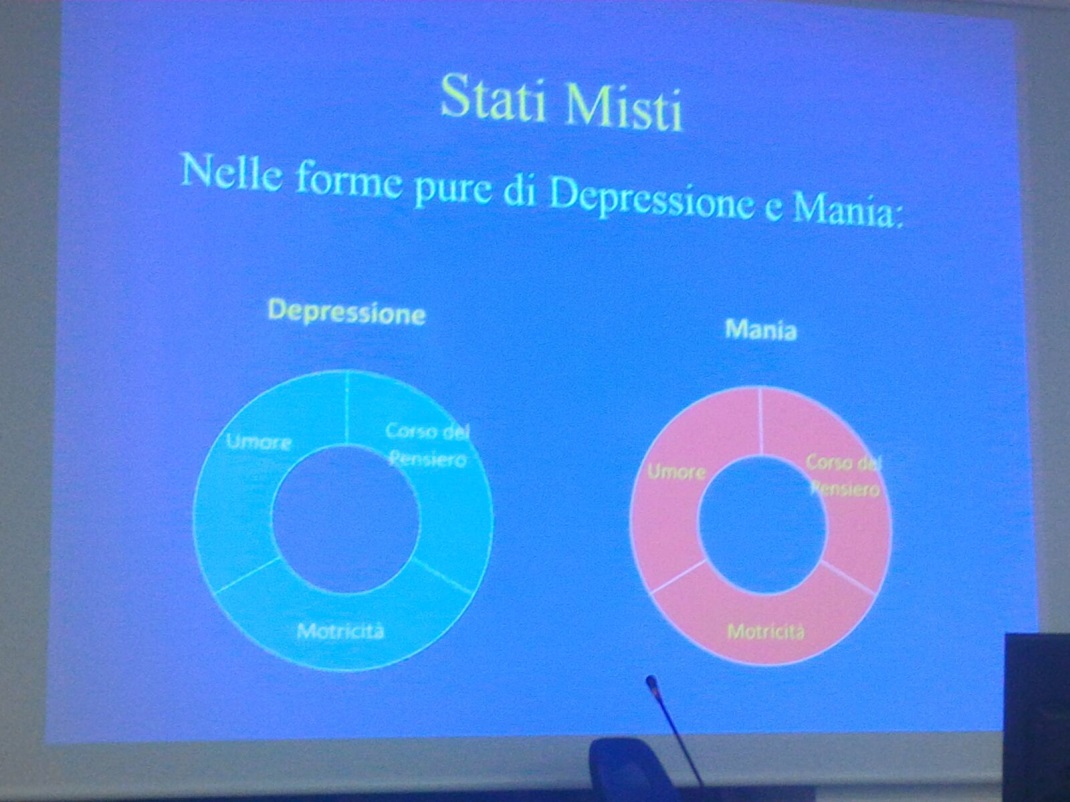
\includegraphics[width=0.9\textwidth]{02/image10.jpeg}
\end{figure}

N\emph{egli stati misti}, invece, \emph{due dei tre elementi sono
concordi per polarità, mentre uno ha polarità opposta}, per cui vi sono
essenzialmente 6 combinazioni principali:


\begin{table}
%\caption{Please write your table caption here}
\begin{tabular}{p{0.5\textwidth}p{0.5\textwidth}}

Mania depressiva		&	Tono dell’umore depresso, ma con ideazione e motilità aumentate \\
Mania acinetica		&	Tono dell’umore aumentato, ideazione accelerata, ma riduzione della motilità  \\
Depressione con fuga delle idee	&	Tono dell’umore depresso, motilità ridotta, ma ideazione aumentata \\
Mania improduttiva	&	Tono dell’umore elevato, motilità aumentata, ma ideazione ridotta \\
Depressione Agitata	&	Tono dell’umore depresso, ideazione inibita, ma motilità aumentata \\
Stupor Maniacale		&	Tono dell’umore elevato,  ma motilità ed ideazione ridotte \\

\noalign{\smallskip}\hline\noalign{\smallskip}
\end{tabular}
\end{table}


\begin{figure}[!ht]
\centering
	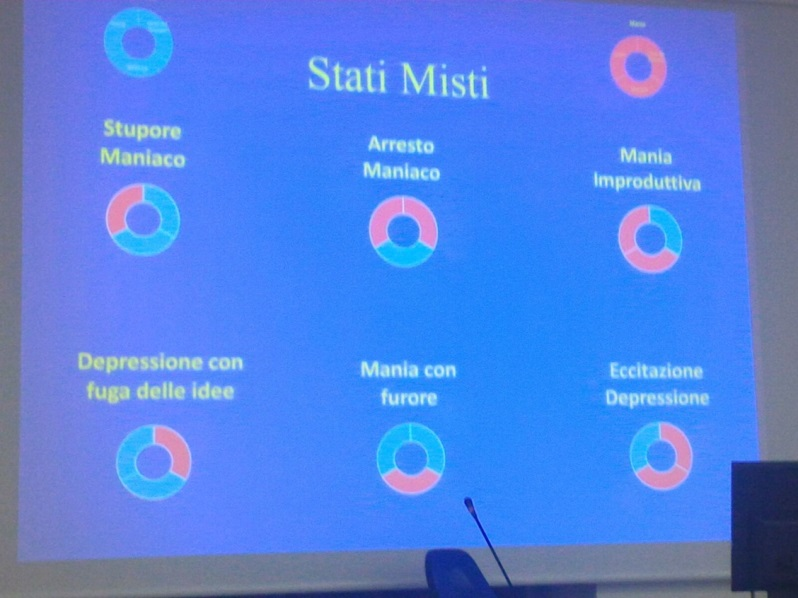
\includegraphics[width=0.9\textwidth]{02/image11.jpeg}
\end{figure}

Gli stati misti possono poi essere suddivisi in \textbf{STABILI} ed
\textbf{INSTABILI} in base alla \emph{comparsa di variazioni
persistenti} (stabili) \emph{o di viraggi rapidamente alternantisi}
(instabili) \emph{a carico dell'affettività}, \emph{dell'energia vitale
e della risonanza affettiva}.

Spesso si possono poi avere delle \textbf{alterazioni del bioritmo},
come disturbi del sonno o variazioni diurne o quasi circadiane dei
parametri prima descritti.

Forme particolari di disturbi bipolari sono poi lo \textbf{stato misto
maniaco-depressivo}, che si caratterizza per la presenza di
\emph{fenomeni dispercettivi}, \emph{idee deliranti}, \emph{alterazioni
della coscienza spesso indistinguibili da quelli della demenza praecox},
ed il \textbf{disturbo bipolare a cicli rapidi}, caratterizzato dalla
presenza di \emph{almeno 4 episodi di alterazione dell'umore nei 12 mesi
precedenti}, che soddisfano i criteri per un episodio depressivo
maggiore, maniacale, misto o ipomaniacale, i quali sono \emph{demarcati
da una remissione parziale o completa per almeno 2 mesi}, o da un
viraggio verso un episodio di opposta polarità.
\end{itemize}

\textbf{Di seguito una serie di casi clinici esemplificativi dei
disturbi visti:}

\emph{Caso clinico 1:}

Pz che diceva di essere ``l'anti-cristo'' (usando questo termine
intendendo di essere il ``secondo cristo'', quindi un salvatore del
mondo - mania), ma dopo poche ore lo ritrovavamo che affermava di essere
incapace e indegno \textbf{stato misto instabile}.

\emph{Caso clinico 2:}

Pz ricoverata, 38 anni, che è convinta di essere la Madonna. Dice che da
piccola era stata ricoverata in pediatria e che di fianco a lei c'era
una bambina con un cappotto rosso e che lei non ha più visto, e afferma
che: ``non so se è perché l'hanno buttata dalla finestra o se perché mi
hanno buttato dalla finestra. Però penso di averla ritrovata..'' e
indica la sua vicina di letto (ma non è possibile dato che ha 20 anni in
più di lei). La pz poi di notte vaga per il reparto, presa da frenesia,
ma alla mattina non lo ricorda, non ricorda nemmeno di aver preso le
gocce alla sera. Lei è convita che questo sia un effetto collaterale dei
farmaci (acatisia in effetti può esserlo) ma non è possibile che si
manifesti solo di sera!

Da questo si è capito che, probabilmente, dato che lei tende ad
oscillare nell'umore, di notte è agitata e si trova in uno stato molto
particolare, un po' come soggetti anziani con demenza che vanno incontro
a confusione soprattutto di notte. La pz ha queste alterazioni molto
particolari: se non si fa attenzione si potrebbe sbagliare la diagnosi,
pensando a schizofrenia o a un quadro di compromissione cerebrale grave.

\emph{Caso clinico 3:}

Signora di 50 anni, che vestiva sempre in grigio o nero. Un giorno si
presenta vestita in modo eccentrico (camicia hawaiana, gonna fucsia,
cappellino, infradito) era cambiata la fase di malattia. Afferma che
sarebbe atterato un elicottero e che l'avrebbero portata in
spiaggia\ldots{}

Questo per dire che per capire se il pz è nella fase maniacale non c'è
particolarmente bisogno di parlare con lui\ldots{}è evidente!

\emph{Caso clinico 4:} in cui pz si presenta in day hospital vestito
come nativo indiano, con penna in testa e lenzuolo attorno alla
vita\ldots{}e nella schiena era pieno di tagli perché si era grattato
con un coltello!

\emph{Caso clinico 5:} il paziente era indeciso se alle olimpiadi fare i
100 m o baseball, e in questo dissidio faceva 10 min di corsa e 10
giocando con la palla\ldots{}

\emph{Caso clinico 6:} il paziente disegnava su fogli un progetto per un
macchinario in grado di spostare la casa da un punto ad un altro perché
era convinto che spostando la casa di 50 metri sarebbe stata più bella
la locazione.

\subsubsection{Distimia}

Mentre nella depressione maggiore e nel disturbo bipolare le fasi di
malattia durano qualche mese (5-6 mesi), poi abbiamo un ritorno
all'eutimia e poi di nuovo un altro episodio; nella distimia invece
abbiamo un disturbo che ha una durata molto più lunga.

È una delle forme di \emph{disturbo dell'umore ad andamento cronico},
anch'essa piuttosto frequente, che secondo i criteri del DSM-IV si
contraddistingue per la \emph{presenza di umore depresso per quasi tutto
il giorno, quasi ogni giorno, per un periodo di almeno due anni},
associato a \emph{due o più dei seguenti sintomi}:

\begin{itemize}
\item
  \textbf{Scarso appetito} o \textbf{iperfagia};
\item
  \textbf{Insonnia} o \textbf{ipersonnia};
\item
  \textbf{Scarsa energia} o \textbf{astenia};
\item
  \textbf{Bassa autostima};
\item
  \textbf{Difficoltà a concentrarsi o nel prendere decisioni};
\item
  \textbf{Sentimenti di disperazione}.
\end{itemize}

Inoltre, durante i due anni di malattia, il soggetto \emph{non deve mai
essere stato privo di sintomi per più di 2 mesi}, e durante il periodo
di malattia \emph{non si devono avere episodi depressivi maggiori
(}tende ad oscillare in prossimità dell'umore normale), così come non
deve essere \emph{mai stato presente un episodio maniacale, misto o
ipomaniacale}, né sono mai stati soddisfatti i criteri per il disturbo
ciclotimico, ed i sintomi devono causare un disagio clinicamente
significativo o una compromissione del funzionamento sociale, lavorativo
o di altre aree importanti.

Bisogna fare quindi molta attenzione, perché prima dell'insorgere del
disturbo distimico può esserci stato un episodio depressivo maggiore,
purché seguito da una remissione totale (cioè senza sintomi per almeno 2
mesi); inoltre, dopo i primi 2 anni (1 solo anno per bambini o
adolescenti) di disturbo distimico possono esserci degli episodi
depressivi maggiori sovrapposti, condizione nota come
``\textbf{\emph{depressione doppia}}'', e la diagnosi viene posta a
seguito del soddisfacimento dei criteri per la depressione maggiore in
paziente già affetto da disturbo distimico. In questo caso, il DSM
raccomanda di riportare se si tratta di una forma ad \emph{esordio
precoce} (sotto i 21 anni), ad \emph{esordio tardivo} (dopo i 21 anni) o
se sono presenti manifestazioni \emph{psicotiche}.

\subsubsection{Ciclotimia}

E\textbf{'}un disturbo che ha sempre una durata estremamente lunga,
almeno 2 anni in cui il soggetto oscilla sia sul versante depressivo,
lieve, sia sul versante ipomaniacale, sfumato, e per due anni continua
in questa oscillazione.

\emph{\textbf{Alcune domande d'esame}} potrebbero essere:

\begin{itemize}
\item[1.]
  quante forme depressive conoscete?
\item[2.]
  Quanti disturbi bipolari conoscete?
\item[3.]
  Un paziente con disturbo bipolare che possibilità ha di avere una vita
  normale?
\end{itemize}
